\documentclass[12pt, a4paper]{report}

\usepackage[T1]{fontenc}
\usepackage[utf8]{inputenc}
\usepackage[romanian]{babel}
\usepackage{geometry}
\geometry{top=2.5cm, bottom=2.5cm, left=3cm, right=2.5cm}
\usepackage{hyperref}
\usepackage{cite}
\usepackage{indentfirst}
\usepackage{amsmath}
\usepackage{xcolor}
\usepackage{listings}
\usepackage{graphicx}
\usepackage{tikz}
\usetikzlibrary{positioning,arrows.meta,shapes.geometric,fit,backgrounds,calc}

% Stil minimal pentru listings (cod sursă)
\definecolor{lstbg}{gray}{0.96}
\definecolor{lstcomment}{rgb}{0.35,0.35,0.35}
\definecolor{lstkeyword}{rgb}{0.0,0.0,0.55}
\lstset{
  backgroundcolor=\color{lstbg},
  basicstyle=\ttfamily\footnotesize,
  commentstyle=\color{lstcomment}\itshape,
  keywordstyle=\color{lstkeyword}\bfseries,
  numbers=none,
  frame=single,
  framerule=0.2pt,
  rulecolor=\color{black!30},
  breaklines=true,
  breakatwhitespace=true,
  showstringspaces=false,
  captionpos=b,
  belowcaptionskip=0.4em,
  aboveskip=0.6em,
  belowskip=0.6em,
  xleftmargin=0.5em,
  xrightmargin=0.5em,
}

\begin{document}

% ── Pagina de titlu ──────────────────────────────────────────
\begin{titlepage}
  \centering

  \textsc{Universitatea Babeș-Bolyai Cluj-Napoca}\\
  \textsc{Facultatea de Matematică și Informatică}\\
  \textsc{Specializarea Informatică în Limba Română}

  \vspace{5cm}

  {\Large LUCRARE DE LICENȚĂ}

  \vspace{1.5cm}

  {\large\itshape Kernel Trap: Sistem Inteligent de Prevenire\\
  a Intruziunilor cu Componente de Honeypot\\
  și Învățare Automată}

  \vfill

  \begin{minipage}{0.45\textwidth}
    \flushleft
    Coordonator\\
    Conf. Univ. Dr. \textit{Bufnea Darius Vasile}
  \end{minipage}
  \hfill
  \begin{minipage}{0.45\textwidth}
    \flushright
    Autor\\
    Banciu George-Horațiu
  \end{minipage}

  \vspace{2cm}
  2026

\end{titlepage}
% ── Abstract ──────────────────────────────────────────────────

\newpage
\begin{center}
  {\large\bfseries Abstract}
\end{center}
\vspace{0.5cm}

Sistemele de detectare a intruziunilor bazate pe gazdă (HIDS) și honeypot-urile
sunt două abordări complementare în apărarea cibernetică, însă utilizate izolat
suferă de limitări semnificative: primele generează alerte fără un mecanism
automat de răspuns, iar cele din urmă sunt pasive, întrucât un atacator care a
compromis deja un sistem nu are niciun motiv să migreze voluntar către o
capcană. Lucrarea de față prezintă KernelTrap, un sistem distribuit care
integrează cele două abordări într-un singur flux automat. Sistemul
monitorizează apelurile de sistem produse de sesiunile SSH active prin
tehnologia eBPF, evaluează fiecare eveniment cu un model Isolation Forest
antrenat pe setul de date BETH și, atunci când o fereastră glisantă 
semnalează un nivel critic de anomalii, redirecționează transparent
sesiunea atacatorului către un container Docker honeypot.
Rezultatele experimentale pe scenarii reale de atac confirmă fezabilitatea
abordării, cu un overhead sub 2,5\% pe CPU pe gazda monitorizată.

\newpage
% ── Cuprins ──────────────────────────────────────────────────
\tableofcontents
\newpage

% ── Capitole ─────────────────────────────────────────────────
\chapter{Introducere}

Creșterea numărului de amenințări cibernetice și sofisticarea atacurilor direcționate impun soluții de securitate capabile să depășească limitele modelelor tradiționale de detecție. 
Sistemele de detectare a intruziunilor bazate pe gazdă (\textit{Host-based Intrusion Detection Systems}, HIDS) oferă un strat de apărare cu granularitate ridicată, 
monitorizând evenimentele produse direct pe sistemul de operare al mașinii țintă~\cite{liu2018hids}. Printre sursele de telemetrie disponibile, apelurile de sistem (\textit{syscalls}) 
reprezintă cea mai fidelă oglindă a comportamentului proceselor, deoarece orice acțiune relevantă pentru securitate, crearea de procese, accesul la fișiere,
comunicația prin rețea, trece obligatoriu prin această interfață. Metodele de învățare automată aplicate pe secvențe de syscall-uri depășesc abordările clasice bazate pe semnături, 
deoarece pot detecta și atacuri necunoscute anterior (\textit{zero-day})~\cite{ring2021deep}; 
compromisul acceptat este o rată mai mare de fals pozitive, care trebuie gestionată prin mecanisme suplimentare de agregare.

O categorie complementară de apărare o constituie honeypot-urile, sisteme-capcană proiectate să atragă atacatorii într-un mediu controlat, 
izolat de resursele reale. Abordările tradiționale de honeypot sunt însă pasive: atacatorul trebuie să ajungă la capcană din proprie inițiativă, 
ceea ce nu se întâmplă dacă a compromis deja un sistem legitim. Lucrarea de față pornește de la această limitare și propune \textbf{KernelTrap}: 
un sistem activ de prevenire a intruziunilor care, în momentul în care detectează un comportament anormal, redirecționează transparent sesiunea SSH a 
atacatorului către un container honeypot dedicat, fără a-l avertiza.

Bazat pe o analiză a literaturii de specialitate și a tehnologiilor disponibile, sistemul KernelTrap integrează trei niveluri funcționale:
colectarea evenimentelor de syscall prin intermediul tehnologiei \textit{extended Berkeley Packet Filter} (eBPF) cu instrumentul Tracee, 
analiza centralizată bazată pe algoritmul Isolation Forest antrenat pe setul de date BETH, și un mecanism de răspuns activ care combină semnale POSIX,
containere Docker și reguli \texttt{iptables}.

Lucrarea este organizată în șapte capitole, după cum urmează:

- Capitolul 1 prezintă contextul problemei, motivația și contribuțiile principale ale lucrării.

- Capitolul 2 introduce conceptele teoretice necesare înțelegerii sistemului: apelurile de sistem și rolul lor în securitate, 
tehnologia eBPF și Tracee, algoritmul Isolation Forest, Redis Streams și containerizarea Docker.

- Capitolul 3 analizează lucrările relevante din domeniu, acoperind HIDS bazate pe syscall-uri~\cite{liu2018hids}, 
metode de învățare automată aplicate la detectarea intruziunilor~\cite{ring2021deep}, precum și soluțiile existente de tip honeypot și limitările acestora.

- Capitolul 4 descrie arhitectura detaliată a sistemului KernelTrap: deciziile de proiectare, protocoalele de comunicație inter-componente și fluxul de date de la colectare până la răspuns.

- Capitolul 5 prezintă implementarea concretă a fiecărei componente: agentul de colectare, serverul central de analiză și mecanismul de pivotare către honeypot.

- Capitolul 6 prezintă evaluarea experimentală a sistemului: metrici de performanță, scenarii reale de atac cu unelte publice și limitările asumate ale domeniului de aplicabilitate.

- Capitolul 7 sintetizează contribuțiile lucrării și propune direcții de extindere ulterioară a sistemului.

\vspace{1em}
În procesul de elaborare a acestei lucrări, autorul a utilizat modele lingvistice generative, în special ChatGPT și Claude Code,
 pentru asistarea completării unor fragmente de cod, generarea unor versiuni inițiale ale codului și, ocazional, reformularea unor enunțuri pentru sporirea clarității.
  După utilizarea acestor instrumente, conținutul a fost revizuit și editat de autor, care își asumă întreaga responsabilitate pentru forma finală și pentru conținutul tezei.

% ================================================================
% Capitolul 2 – Aspecte Teoretice
% Lucrare de licență: Kernel Trap – Sistem Inteligent de Prevenire
% a Intruziunilor cu Componente de Honeypot și Învățare Automată
% Autor: Banciu George-Horațiu
% Coordonator: Conf. Univ. Dr. Bufnea Darius Vasile
% ================================================================

\chapter{Aspecte teoretice}

Capitolul de față prezintă fundamentele conceptuale și tehnologice pe care se construiesc
sistemele moderne de detectare și prevenire a intruziunilor bazate pe monitorizarea la nivel
de kernel. Sunt tratate paradigmele IDS/IPS, mecanismele de interceptare a apelurilor de sistem
prin eBPF, instrumentele de colectare a evenimentelor, tehnicile de detecție a anomaliilor prin
învățare automată nesupervizată și principiile apărării active prin honeypot-uri.

% ----------------------------------------------------------------
\section{Sisteme de detectare și prevenire a intruziunilor}
% ----------------------------------------------------------------

Un \textit{sistem de detectare a intruziunilor} (\textit{Intrusion Detection System}, IDS) este
o componentă de securitate ce monitorizează în timp real activitatea unui sistem sau rețea în scopul
identificării comportamentelor suspecte sau a activităților neautorizate~\cite{liu2018hids}. Atunci
când un IDS este dotat și cu capacități de răspuns activ (blocarea conexiunilor, terminarea
proceselor sau redirecționarea traficului), acesta devine un \textit{sistem de prevenire a
intruziunilor} (\textit{Intrusion Prevention System}, IPS).

Din perspectiva punctului de colectare a datelor, sistemele IDS se clasifică în două mari categorii:

\begin{itemize}
  \item NIDS (\textit{Network-based IDS}): monitorizează traficul de rețea la nivel de
    pachete, identificând tipare de atac (scanări de porturi, flood-uri, exploit-uri cunoscute)
    fără acces la starea internă a gazdelor individuale.
  \item HIDS (\textit{Host-based IDS}): rulează direct pe gazda monitorizată și analizează
    evenimente produse la nivelul sistemului de operare (apeluri de sistem, jurnale de aplicație,
    accesuri la fișiere și modificări de configurație), oferind vizibilitate asupra comportamentului
    proceselor individuale~\cite{liu2018hids}.
\end{itemize}

Cele două abordări sunt complementare: NIDS detectează atacuri la nivel de transport, dar nu poate
inspecta comunicațiile criptate și nu are acces la comportamentul intern al proceselor; HIDS are
vizibilitate deplină asupra stării gazdei, dar nu observă activitatea laterală dintre alte mașini
din rețea.

Literatura de specialitate distinge două paradigme principale de detecție~\cite{liu2018hids,ring2021deep}:

\textbf{Detecția bazată pe semnături} (\textit{signature-based detection}) compară activitatea
observată cu o bază de cunoștințe de tipare de atac cunoscute. Rata de fals pozitive este scăzută
iar detecția este rapidă, dar metoda este prin definiție oarbă la amenințările noi (\textit{zero-day})
care nu figurează în baza de semnături. Soluții comerciale precum Snort sau Suricata se bazează
preponderent pe această abordare.

\textbf{Detecția bazată pe anomalii} (\textit{anomaly-based detection}) construiește un model al
comportamentului normal și semnalează orice deviere semnificativă de la acesta. Această paradigmă
poate detecta, în principiu, atacuri necunoscute anterior, deoarece nu depinde de semnăturile lor
specifice. Compromisul acceptat constă într-o rată mai ridicată de fals pozitive, generată de
variabilitatea naturală a comportamentului benign. Sistemele moderne combină adesea ambele abordări
pentru a valorifica avantajele fiecăreia~\cite{ring2021deep}.

% ----------------------------------------------------------------
\section{Apeluri de sistem și rolul lor în securitate}
% ----------------------------------------------------------------

Sistemul de operare Linux separă execuția în \textit{user space} (unde rulează aplicațiile
neprivilegiate) și \textit{kernel space}, unde se execută codul privilegiat al nucleului.
Această separare este impusă hardware prin inelele de protecție ale procesorului (Ring 0 pentru
kernel, Ring 3 pentru aplicații) și constituie fundația modelului de securitate al sistemului
de operare~\cite{bovet2005understanding}.

Comunicarea dintre cele două domenii se realizează exclusiv prin \textit{apeluri de sistem}
(\textit{syscalls}): puncte de intrare controlate prin care un program solicită nucleului operații
privilegiate. Nucleul Linux expune în prezent peste 300 de apeluri de sistem, grupate funcțional
în categorii: gestionarea proceselor (\texttt{fork}, \texttt{execve}, \texttt{exit}), accesul la
fișiere (\texttt{open}, \texttt{read}, \texttt{write}, \texttt{unlink}), comunicația prin rețea
(\texttt{socket}, \texttt{connect}, \texttt{bind}), gestionarea utilizatorilor și privilegiilor
(\texttt{setuid}, \texttt{setgid}, \texttt{capset}) și controlul proceselor
(\texttt{kill}, \texttt{ptrace})~\cite{kerrisk2010linux}.

Orice acțiune relevantă din perspectiva securității trece obligatoriu prin interfața syscall.
Un atacator care rulează un exploit, escaladează privilegii sau exfiltrează date nu poate ocoli
această interfață, indiferent de tehnica folosită. Această proprietate face din secvențele de
syscall-uri o sursă ideală de telemetrie pentru sistemele HIDS.

Spre deosebire de logurile aplicative (care pot fi falsificate sau suprimate de un atacator cu
privilegii ridicate), evenimentele de la nivelul syscall-urilor sunt inspecționate de nucleu
înainte ca aplicația să aibă posibilitatea de a interveni~\cite{tracee2024}. Astfel, chiar dacă
un atacator compromite complet o aplicație, comportamentul acesteia rămâne vizibil prin
instrumentarea nucleului.

Din perspectiva unui HIDS, secvențele de syscall-uri permit identificarea unor tipare
comportamentale caracteristice atacurilor: un \texttt{execve} urmat imediat de \texttt{setuid}
și \texttt{capset} sugerează o tentativă de escaladare de privilegii; o explozie de apeluri
\texttt{connect} către adrese IP externe indică o potențială activitate de tip Command and Control;
o secvență \texttt{open}/\texttt{read} pe fișierele \texttt{/etc/shadow} sau \texttt{/etc/passwd}
semnalează recunoaștere locală a sistemului~\cite{liu2018hids}.

% ----------------------------------------------------------------
\section{Extended Berkeley Packet Filter (eBPF)}
% ----------------------------------------------------------------

Berkeley Packet Filter (BPF), introdus în 1992 de McCanne și Jacobson ca mecanism de filtrare
a pachetelor de rețea la nivel de kernel~\cite{mccanne1993bsd}, a fost extins radical începând
cu nucleul Linux 3.18 (2014) sub forma \textit{extended BPF} (eBPF)~\cite{gregg2019bpf}. Dacă
BPF-ul clasic opera exclusiv pe pachete de rețea, eBPF permite atașarea de programe la orice
punct de instrumentare din nucleu: syscall-uri, kprobes, uprobes, tracepoints și evenimente LSM
(\textit{Linux Security Modules}).

Arhitectural, eBPF funcționează ca o mașină virtuală ușoară integrată în nucleu, cu un set de
instrucțiuni propriu (64 de biți, 11 regiștri generali) și un model de execuție bazat pe evenimente.
Programele sunt scrise în C restricționat, compilate în bytecode și supuse unui \textit{verificator
static} care garantează absența buclelor infinite, a acceselor invalide la memorie și a scurgerilor
de resurse~\cite{gregg2019bpf}. Verificatorul analizează toate căile posibile de execuție
ale programului înainte de încărcare, respingând programele care nu pot fi demonstrate sigure.
Bytecode-ul validat este ulterior compilat JIT (\textit{Just-in-Time}) în instrucțiuni native ale
procesorului.

Starea este partajată între programe și user space prin \textit{eBPF Maps}, structuri cheie-valoare
rezidente în kernel space, accesibile din ambele domenii. Apelurile din programele eBPF către
funcțiile nucleului se fac exclusiv prin \textit{helper functions} cu interfață stabilă, garantând
compatibilitatea între versiuni diferite de kernel. Figura~\ref{fig:cap2-ebpf} sintetizează acest
flux, de la apelul de sistem produs în spațiul utilizator până la citirea evenimentului filtrat,
într-un map, de către un agent din spațiul utilizator precum Tracee.

\begin{figure}[h]
  \centering
  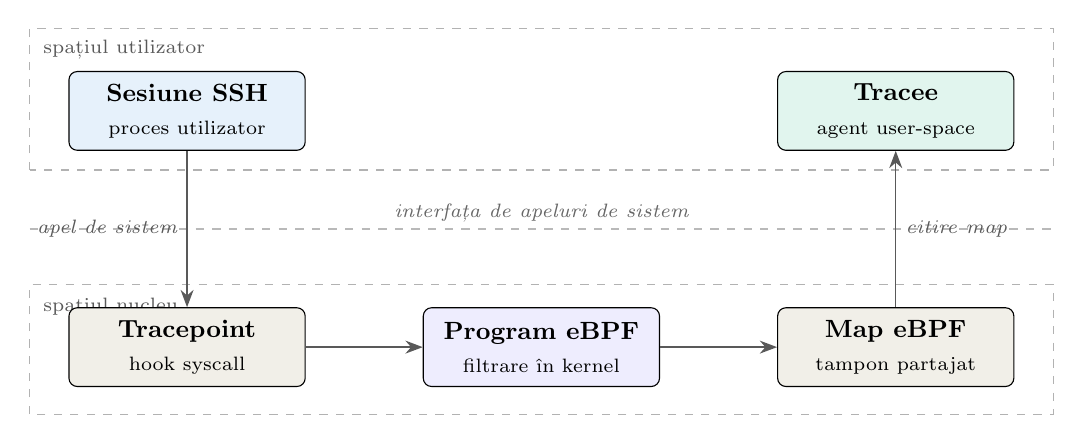
\begin{tikzpicture}[
      font=\small,
      box/.style={rectangle, rounded corners=3pt, draw, line width=0.4pt,
        minimum width=3cm, minimum height=1cm, align=center, inner sep=3pt},
      flow/.style={-{Stealth[length=2.2mm]}, line width=0.5pt, gray!70!black},
      lbl/.style={font=\scriptsize\itshape, text=black!65},
    ]
    \definecolor{cap2ssh}{RGB}{230,241,251}
    \definecolor{cap2tracee}{RGB}{225,245,238}
    \definecolor{cap2gray}{RGB}{241,239,232}
    \definecolor{cap2prog}{RGB}{238,237,254}

    \draw[dashed, gray!60, line width=0.4pt] (-2,-0.75) rectangle (11,1.05);
    \node[anchor=north west, font=\scriptsize, text=gray!70!black] at (-1.95,1.02) {spațiul utilizator};
    \draw[dashed, gray!60, line width=0.4pt] (-2,-3.85) rectangle (11,-2.2);
    \node[anchor=north west, font=\scriptsize, text=gray!70!black] at (-1.95,-2.25) {spațiul nucleu};
    \draw[dashed, gray!55, line width=0.4pt] (-2,-1.5) -- (11,-1.5);
    \node[font=\scriptsize\itshape, text=black!60] at (4.5,-1.3) {interfața de apeluri de sistem};

    \node[box, fill=cap2ssh]    (ssh)    at (0,0)    {\textbf{Sesiune SSH}\\[1pt]\scriptsize proces utilizator};
    \node[box, fill=cap2tracee] (tracee) at (9,0)    {\textbf{Tracee}\\[1pt]\scriptsize agent user-space};
    \node[box, fill=cap2gray]   (tp)     at (0,-3)   {\textbf{Tracepoint}\\[1pt]\scriptsize hook syscall};
    \node[box, fill=cap2prog]   (prog)   at (4.5,-3) {\textbf{Program eBPF}\\[1pt]\scriptsize filtrare în kernel};
    \node[box, fill=cap2gray]   (map)    at (9,-3)   {\textbf{Map eBPF}\\[1pt]\scriptsize tampon partajat};

    \draw[flow] (ssh.south) -- node[lbl, left] {apel de sistem} (tp.north);
    \draw[flow] (tp.east) -- (prog.west);
    \draw[flow] (prog.east) -- (map.west);
    \draw[flow] (map.north) -- node[lbl, right] {citire map} (tracee.south);
  \end{tikzpicture}
  \caption[Fluxul de colectare prin eBPF]{Fluxul de colectare prin eBPF. Un apel de sistem produs de o sesiune SSH traversează
  interfața de apeluri de sistem; în nucleu, un program eBPF atașat la un tracepoint filtrează
  evenimentul și îl scrie într-un map, de unde agentul Tracee îl citește în spațiul utilizator.}
  \label{fig:cap2-ebpf}
\end{figure}

Înainte de eBPF, instrumentarea nucleului la runtime necesita una din două abordări, ambele
problematice în producție: modificarea codului sursă al nucleului (imposibilă fără acces la sursă
și fără repornire) sau încărcarea de module de nucleu (\textit{Loadable Kernel Modules}, LKM).
Modulele de nucleu rulează în Ring 0, fără niciun mecanism de verificare prealabilă, iar un bug
poate produce panică de kernel sau compromiterea întregului sistem.

eBPF elimină aceste limitări: programele se încarcă la runtime, fără repornire, și sunt garantate
sigure de verificator înainte de execuție. Față de mecanisme alternative precum \texttt{auditd}
sau \texttt{ptrace}, eBPF prezintă cost suplimentar semnificativ mai redus, deoarece filtrarea și
agregarea evenimentelor se realizează direct în kernel space, reducând la minimum cantitatea de
date transferate către user space~\cite{gregg2019bpf}.

% ----------------------------------------------------------------
\section{Tracee: instrumentul de colectare a evenimentelor}
% ----------------------------------------------------------------

Tracee este un instrument open-source de securitate runtime pentru Linux, dezvoltat și menținut
de Aqua Security~\cite{aqua2024tracee}. Folosește eBPF pentru a intercepta evenimentele de sistem
la runtime și a le expune ca fluxuri de date structurate în format JSON, acoperind un spectru larg
de activitate: crearea și terminarea de procese, accesul la fișiere, conexiunile de rețea,
modificările de permisiuni și evenimentele LSM.

Tracee este compus din două componente principale: \textbf{Tracee-eBPF}, care compilează și
încarcă programele eBPF în nucleu și expune fluxul brut de evenimente, și \textbf{Tracee-Rules},
un motor de detectare bazat pe reguli scrise în Go sau Rego (limbajul de politici al Open Policy
Agent). O caracteristică notabilă este preferința pentru evenimentele
LSM față de syscall-urile brute (de exemplu, \texttt{security\_file\_open} în locul \texttt{openat}),
care oferă informații mai complete despre contextul de securitate și sunt mai puțin susceptibile
la atacuri de tip TOCTOU (\textit{Time-of-Check to Time-of-Use})~\cite{aqua2024tracee}.

Portabilitatea pe kernel-uri diferite este asigurată prin suportul \textit{Compile Once – Run
Everywhere} (CO:RE), bazat pe \textit{BPF Type Format} (BTF): pe nucleele cu BTF activat, nu
sunt necesare nici recompilarea probe-urilor, nici prezența header-elor de nucleu pe sistemul
țintă. Aceasta face din Tracee o soluție practică pentru deployment pe
infrastructuri eterogene.

% ----------------------------------------------------------------
\section{Honeypot-uri și apărarea activă}
% ----------------------------------------------------------------

Un \textit{honeypot} este un sistem de securitate proiectat deliberat să fie compromis, cu scopul
de a atrage atacatorii, de a le studia tehnicile și de a le deturnă resursele și atenția de la
sistemele reale~\cite{spitzner2002honeypots}. Spre deosebire de sistemele de producție, un honeypot
nu conține date sau servicii reale, iar orice interacțiune cu el este, prin definiție, suspectă.

Taxonomia standard clasifică honeypot-urile după două criterii principale:

\textbf{Nivelul de interacțiune} distinge între:
\begin{itemize}
  \item \textit{Honeypot-uri cu interacțiune redusă} (\textit{low-interaction}): emulează servicii
    și sisteme de operare fără a rula un sistem real. Sunt ușor de implementat și cu risc minim
    de compromitere, dar oferă informații limitate despre tehnicile atacatorului. Exemple tipice:
    Honeyd, OpenCanary.
  \item \textit{Honeypot-uri cu interacțiune ridicată} (\textit{high-interaction}): expun sisteme
    reale (sau mașini virtuale complete) cu servicii funcționale. Colectează informații detaliate
    despre comportamentul atacatorului, inclusiv tool-uri folosite, comenzi executate și ținte
    vizate ulterior, dar prezintă risc mai ridicat dacă atacatorul reușește să evadeze din
    mediul controlat~\cite{spitzner2002honeypots}.
\end{itemize}

\textbf{Scopul de utilizare} distinge între:
\begin{itemize}
  \item \textit{Honeypot-uri de cercetare}: implementate de organizații de securitate pentru
    studierea tehnicilor de atac emergente, colectarea de mostre de malware și înțelegerea
    comportamentului atacatorilor.
  \item \textit{Honeypot-uri de producție}: integrate în rețelele organizațiilor pentru a detecta
    activitate neautorizată internă și a alerta echipele de securitate.
\end{itemize}

Honeypot-urile tradiționale funcționează pasiv: atacatorul trebuie să ajungă la capcană din
proprie inițiativă, alegând să interacționeze cu un serviciu-momeală. Această abordare prezintă
o limitare fundamentală în scenariile în care atacatorul a compromis deja un sistem legitim,
deoarece el nu are niciun motiv să migreze voluntar către un honeypot.

O abordare mai avansată, denumită \textit{apărare activă} (\textit{active deception}), inversează
această logică prin redirecționarea transparentă a unui atacator detectat de pe sistemul compromis
către un honeypot, fără ca acesta să conștientizeze tranziția. Mecanismul se bazează tipic pe
reguli NAT (\texttt{iptables}/\texttt{nftables}), care interceptează traficul la nivel de rețea
și îl deviază înainte ca pachetele să ajungă la destinația originală~\cite{spitzner2002honeypots}.
Avantajul față de abordarea pasivă constă în faptul că atacatorul nu trebuie să aleagă
honeypot-ul din proprie inițiativă, ci este direcționat acolo în momentul în care comportamentul
său declanșează un semnal de alertă, indiferent că a compromis deja un serviciu real.

Un concept complementar honeypot-urilor îl reprezintă \textit{honeytoken-ul}: un artefact digital
fals (fișier, cheie de acces, înregistrare în bază de date) plasat intenționat într-un sistem
real sau într-un honeypot, proiectat să nu fie niciodată accesat de utilizatori legitimi. Orice
interacțiune cu un honeytoken constituie, prin definiție, un indicator incontestabil de
compromitere~\cite{spitzner2002honeypots}. Spre deosebire de detecția bazată pe anomalii
statistice, care produce un scor continuu cu risc de fals pozitive, accesul la un honeytoken
este un semnal binar și precis: niciun utilizator legitim nu are motiv să deschidă un fișier de
credențiale pe care el însuși nu l-a creat. Honeytokens-urile pot lua diverse forme: fișiere cu
credențiale fictive, chei SSH false, token-uri de API nevalide sau înregistrări-capcană în baze
de date. Sunt utilizate atât în medii de producție pentru detectarea accesului neautorizat,
cât și în honeypot-uri pentru a monitoriza comportamentul post-compromitere al atacatorilor.

% ----------------------------------------------------------------
\section{Algoritmul Isolation Forest}
% ----------------------------------------------------------------

Isolation Forest (\textit{iForest}), propus de Liu, Ting și Zhou în 2008~\cite{liu2008iforest},
adoptă o paradigmă diferită față de metodele clasice de detecție a anomaliilor (LOF, k-NN,
One-Class SVM): în loc să modeleze distribuția normală și să identifice instanțele care se
abat de la ea, izolează explicit anomaliile prin partiționări recursive aleatorii.

Intuiția algoritmului se bazează pe două proprietăți ale anomaliilor: acestea sunt \textit{rare}
(puține la număr față de instanțele normale) și \textit{diferite} (ocupă regiuni izolate ale
spațiului de caracteristici). Ca urmare, ele pot fi separate de restul datelor printr-un număr
semnificativ mai mic de partiționări aleatorii decât instanțele normale, care sunt dense și
necesită multe partiționări pentru a fi izolate~\cite{liu2012isolation}
(Figura~\ref{fig:cap2-iforest}).

\begin{figure}[h]
  \centering
  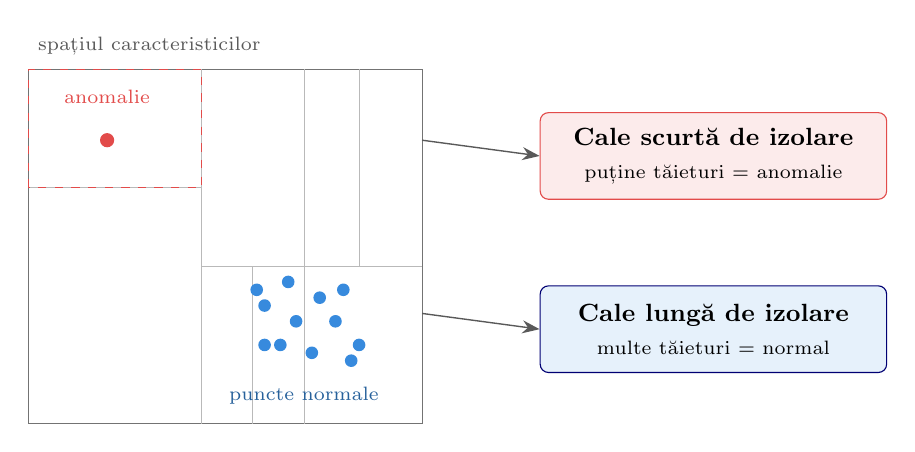
\begin{tikzpicture}[
      font=\small,
      boxc/.style={rectangle, rounded corners=3pt, draw, line width=0.4pt,
        minimum width=4.4cm, minimum height=1.1cm, align=center, inner sep=3pt},
      flow/.style={-{Stealth[length=2.2mm]}, line width=0.5pt, gray!70!black},
    ]
    \definecolor{cap2anom}{RGB}{226,75,74}
    \definecolor{cap2norm}{RGB}{55,138,221}
    \definecolor{cap2redbox}{RGB}{252,235,235}
    \definecolor{cap2bluebox}{RGB}{230,241,251}

    \node[anchor=south west, font=\scriptsize, text=black!65] at (0,4.55) {spațiul caracteristicilor};
    \draw[line width=0.4pt, black!55] (0,0) rectangle (5,4.5);

    \draw[gray!55, line width=0.3pt] (2.2,0) -- (2.2,4.5);
    \draw[gray!55, line width=0.3pt] (0,3.0) -- (2.2,3.0);
    \draw[gray!55, line width=0.3pt] (3.5,0) -- (3.5,4.5);
    \draw[gray!55, line width=0.3pt] (2.2,2.0) -- (5,2.0);
    \draw[gray!55, line width=0.3pt] (4.2,2.0) -- (4.2,4.5);
    \draw[gray!55, line width=0.3pt] (2.85,0) -- (2.85,2.0);

    \draw[cap2anom, dashed, line width=0.5pt] (0,3.0) rectangle (2.2,4.5);
    \fill[cap2anom] (1.0,3.6) circle (0.09);
    \node[font=\scriptsize, text=cap2anom] at (1.0,4.15) {anomalie};

    \foreach \p in {(3.0,1.5),(3.4,1.3),(3.7,1.6),(3.2,1.0),(3.6,0.9),(3.9,1.3),(3.3,1.8),(3.0,1.0),(4.0,1.7),(4.2,1.0),(2.9,1.7),(4.1,0.8)}
      \fill[cap2norm] \p circle (0.08);
    \node[font=\scriptsize, text=cap2norm!70!black] at (3.5,0.35) {puncte normale};

    \node[boxc, fill=cap2redbox,  draw=cap2anom]      (short) at (8.7,3.4) {\textbf{Cale scurtă de izolare}\\[1pt]\scriptsize puține tăieturi = anomalie};
    \node[boxc, fill=cap2bluebox, draw=blue!45!black] (long)  at (8.7,1.2) {\textbf{Cale lungă de izolare}\\[1pt]\scriptsize multe tăieturi = normal};

    \draw[flow] (5,3.6) -- (short.west);
    \draw[flow] (5,1.4) -- (long.west);
  \end{tikzpicture}
  \caption[Intuiția algoritmului Isolation Forest]{Intuiția algoritmului Isolation Forest. O anomalie, situată într-o regiune rară a
  spațiului de caracteristici, este izolată din puține tăieturi aleatorii (cale scurtă în arbore),
  în timp ce un punct dintr-un cluster dens necesită multe tăieturi (cale lungă) pentru a fi
  separat.}
  \label{fig:cap2-iforest}
\end{figure}

Algoritmul construiește o pădure de \textit{isolation trees} (iTrees). Fiecare iTree este un
arbore binar construit prin selecția aleatorie repetată a unui atribut $q$ și a unui prag de
partiționare $p$ ales uniform în intervalul de valori al atributului, până când fiecare instanță
este izolată într-un nod frunză. O pădure constă din $t$ astfel de arbori, fiecare antrenat
pe un subsample de dimensiune $\psi$; valorile implicite sunt $t = 100$, $\psi = 256$~\cite{liu2008iforest}.

Lungimea căii $h(x)$ printr-un iTree reprezintă numărul de muchii parcurse de la rădăcină până
la nodul de izolare al instanței $x$. Anomaliile, mai ușor de izolat, prezintă căi mai scurte;
instanțele normale, mai greu de separat, prezintă căi mai lungi. Scorul de anomalie normalizat
este definit ca:
\[
    s(x, \psi) = 2^{-\dfrac{E[h(x)]}{c(\psi)}}
\]
unde $E[h(x)]$ este media lungimilor de cale pe toți $t$ arborii, iar $c(\psi)$ este lungimea
medie de cale așteptată pentru un arbore binar de căutare construit pe $\psi$
instanțe~\cite{liu2012isolation}. Un scor $s \approx 1$ indică anomalie certă, $s \approx 0.5$
instanță nedistinctivă, iar $s \approx 0$ comportament cu certitudine normal.

Față de metodele bazate pe distanță sau densitate, iForest are complexitate liniară $O(n)$,
memorie redusă prin subsampling fix și nu necesită date etichetate cu atacuri, proprietăți
esențiale într-un context de securitate unde datele de atac sunt rare sau inexistente la
momentul antrenării~\cite{liu2008iforest,liu2012isolation}.

% ----------------------------------------------------------------
\section{Setul de date BETH}
% ----------------------------------------------------------------

Setul de date BETH (\textit{BPF-Extended Tracking Honeypot}), prezentat de Highnam et al. la
ICML Workshop on Uncertainty and Robustness in Deep Learning (2021)~\cite{highnam2021beth}, este
unul dintre puținele seturi de date publice de evenimente de syscall colectate dintr-un scenariu
real de honeypot în mediu cloud. Conține peste 8 milioane de evenimente capturate de pe 23 de
gazde honeypot expuse pe internet timp de mai multe zile.

Fiecare eveniment este reprezentat prin 14 caracteristici brute: \texttt{processId},
\texttt{parentProcessId}, \texttt{userId}, \texttt{mountNamespace}, \texttt{eventId},
\texttt{argsNum}, \texttt{returnValue} și altele, și este etichetat binar: benign (\texttt{evil=0})
sau malițios (\texttt{evil=1}). Setul este partiționat 60/20/20 (antrenament/validare/test);
important, datele de atac apar \textit{exclusiv} în partiția de test, reflectând paradigma
realistă în care un model este antrenat pe comportament benign și evaluat ulterior pe atacuri.
Atacul reprezentat constă în instanțierea unui nod de botnet: exploatare inițială, escaladare
de privilegii și activitate de Command and Control (C\&C).

Față de alte seturi de date sintetice sau de laborator, BETH prezintă avantajul că reflectă
comportamentul real al unui atacator pe servere Linux expuse la internet, colectat prin aceeași
tehnologie eBPF utilizată de instrumentele moderne de monitorizare. Isolation Forest atinge
AUROC de 0.850 pe acest set, cel mai bun rezultat dintre modelele clasice nesupervizate testate
în literatura de specialitate~\cite{highnam2021beth}.

% ----------------------------------------------------------------
\section{Redis Streams}
% ----------------------------------------------------------------

Redis Streams, introdusă în Redis 5.0 (2018), este o structură de date de tip jurnal
\textit{append-only} cu acces aleator în timp $O(1)$, destinată scenariilor de mesagerie și
procesare de evenimente în timp real~\cite{redis2024streams}. Fiecare intrare
(\textit{entry}) dintr-un stream este identificată printr-un ID monoton crescător (compus din
timestamp în milisecunde și un număr de secvență) și conține un set arbitrar de perechi
câmp-valoare.

Spre deosebire de Redis Pub/Sub,care pierde mesajele dacă niciun subscriber nu este activ
în momentul publicării, Streams persistă intrările pe disc și le face disponibile pentru citire ulterioară. Mecanismul de \textit{consumer groups}
permite mai multor consumatori să citească din același stream în paralel, fiecare primind un
subset disjunct de mesaje; un mesaj rămâne în starea \textit{pending} până la confirmarea
explicită prin comanda \texttt{XACK}, garantând că niciun eveniment nu se pierde în caz de
cădere a consumatorului.

Aceste caracteristici fac din Redis Streams o soluție potrivită pentru arhitecturi de tip
pipeline în care un producător de evenimente (agentul de monitorizare) trebuie decuplat de
consumatorul de analiză, cu garanții de livrare și fără introducerea complexității operaționale
a unui broker distribuit dedicat.

% ----------------------------------------------------------------
\section{Containerizarea Docker și rolul în mecanismul honeypot}
% ----------------------------------------------------------------

Docker permite ambalarea unei aplicații împreună cu toate dependențele sale într-o unitate
portabilă și reproductibilă numită \textit{container}~\cite{merkel2014docker}. Spre deosebire
de mașinile virtuale, care virtualizează hardware-ul complet și rulează un nucleu propriu,
containerele partajează nucleul sistemului gazdă și se izolează exclusiv prin mecanisme
software ale nucleului Linux:

\begin{itemize}
  \item \textit{Namespaces}: creează viziuni izolate ale resurselor sistemului pentru fiecare
    container: spații separate de PID (procesele unui container nu pot vedea procesele altui
    container), rețea (interfețe și tabele de rutare proprii), sistem de fișiere
    (\textit{mount namespace}), utilizatori (\textit{user namespace}) și hostname.
  \item \textit{Control groups} (\textit{cgroups}): limitează cantitatea de resurse (CPU,
    memorie, I/O pe disc, lățime de bandă) pe care un container o poate consuma, prevenind
    consumul abuziv al resurselor gazdei.
\end{itemize}

Izolarea prin containere se dovedește utilă și în contextul apărării active: un container
honeypot cu interacțiune ridicată poate expune un shell real și unelte uzuale, simulând un
sistem Linux funcțional, fără ca activitatea atacatorului să afecteze infrastructura de
producție. Tranzițional, regulile NAT (\texttt{iptables}, tabela \texttt{nat}, lanțul
\texttt{PREROUTING}) pot intercepta traficul destinat unui serviciu legitim și îl pot devia
transparent către portul corespunzător al containerului honeypot, înainte ca pachetele să
ajungă la destinația originală. Din perspectiva atacatorului, sesiunea continuă fără întrerupere
vizibilă, dar el interacționează cu un mediu controlat și monitorizat, izolat complet de
sistemele de producție~\cite{spitzner2002honeypots,kerrisk2010linux}.


\chapter{Stadiu actual}
% ================================================================
% Capitolul 3 -- Stadiu actual
% Lucrare de licenta: Kernel Trap -- Sistem Inteligent de Prevenire
% a Intruziunilor cu Componente de Honeypot si Invatare Automata
% Autor: Banciu George-Horatiu
% ================================================================

Capitolul de față trece în revistă stadiul actual al cercetării în domeniile
care converg în arhitectura sistemului propus, evaluează soluțiile existente
și identifică golul pe care lucrarea de față urmărește să îl acopere. KernelTrap
se situează la intersecția a patru direcții de cercetare active în literatura de
specialitate din ultimii ani: monitorizarea comportamentală la nivel de kernel
prin tehnologia eBPF, detectarea anomaliilor pe baza apelurilor de sistem prin
metode de învățare automată nesupervizată, honeypot-urile cu interacțiune
ridicată pentru analiza atacurilor reale și mecanismele de apărare activă
bazate pe redirecționare transparentă a sesiunilor compromise. Pentru fiecare
direcție sunt prezentate atât lucrările fundamentale, cât și contribuțiile
recente (2022--2025), ale căror rezultate fundamentează deciziile de
proiectare expuse în capitolul următor.

\section{Sisteme HIDS bazate pe eBPF}

Tranziția dinspre modulele de nucleu tradiționale (LKM) către programe eBPF
reprezintă cea mai semnificativă schimbare în domeniul
monitorizării de securitate la nivel de gazdă din ultimul deceniu.
Soldani et al.~\cite{soldani2023ebpf} oferă cea mai cuprinzătoare analiză
recentă a tehnologiei eBPF pentru observabilitate cloud-native și securitate
runtime, demonstrând că suprafața redusă de atac, garanțiile statice oferite de
verificator și costul redus de instrumentare fac din eBPF alegerea naturală
pentru sisteme HIDS moderne.
Hao et al.~\cite{hao2024ebpfruntime} descriu în detaliu implementarea
runtime-ului eBPF în nucleul Linux 6.7, confirmând maturitatea ecosistemului ca
platformă stabilă pentru produse de securitate.

În spațiul soluțiilor open-source, patru proiecte domină piața:
\textbf{Falco} (CNCF, originar de la Sysdig), care folosește eBPF pentru
colectare și un motor de reguli declarative pentru detecție;
\textbf{Tetragon} (Cilium/Isovalent), care diferă prin capacitatea de aplicare
sincronă a politicilor direct în kernel space;
\textbf{KubeArmor} (Accuknox), care exploatează BPF-LSM pentru aplicarea de
politici de securitate;
și \textbf{Tracee} (Aqua Security), care a fost adoptat și de KernelTrap
pentru capacitățile sale de tracing fără configurare prealabilă pe nuclee
diferite (CO:RE/BTF).
Syairozi și Arizal~\cite{syairozi2025ebpfcomparative} efectuează cea mai
recentă comparație empirică a acestor sisteme pe un set de atacuri OWASP
Kubernetes Top~10, măsurând timpul mediu până la detecție (MTTD), rata de
detecție, rata de fals pozitive și consumul de resurse.
Concluzia studiului este că Tracee oferă cea mai bună acoperire a evenimentelor
LSM și cea mai mică amprentă pe CPU dintre soluțiile testate, susținând
alegerea făcută în cadrul prezentei lucrări.

Două lucrări recente sunt deosebit de relevante pentru arhitectura KernelTrap.
eBPF-PATROL~\cite{ebpfpatrol2025} propune un agent runtime ușor pentru
interceptarea apelurilor de sistem și aplicarea de politici, raportând un
overhead sub 2,5\% un punct de referință apropiat de obiectivele de
performanță ale agentului din KernelTrap.
CryptoGuard~\cite{cryptoguard2024}, publicat la DSN 2024, combină monitorizarea
cu fereastră glisantă a syscall-urilor cu o rețea neuronală evaluată direct în
kernel, atingând un overhead remarcabil de 0,06\% pe CPU.
Aceste lucrări demonstrează fezabilitatea sistemelor HIDS de tip
\textit{always-on} în medii de producție, însă niciuna nu integrează un
mecanism de răspuns activ comparabil cu pivotarea propusă de KernelTrap.

O contribuție notabilă este lucrarea fundamentală a lui Fournier et
al.~\cite{fournier2021ebpf} de la Datadog, care discută în detaliu
compromisurile dintre kprobe-uri, tracepoint-uri și hook-urile LSM, precum și
problemele de tip TOCTOU (\textit{Time-of-Check to Time-of-Use})~ aspecte
direct relevante pentru proiectarea agentului KernelTrap.

\section{Învățare automată nesupervizată pentru detectarea intruziunilor}

Limitările abordărilor supervizate aplicate la detectarea intruziunilor sunt
bine documentate în literatură.
Zoppi și Ceccarelli~\cite{zoppi2022unsupervised,zoppi2022stacking} argumentează 
că modelele bazate pe semnături și clasificatorii binari
supervizați eșuează sistematic la detectarea atacurilor zero-day, întrucât
distribuția datelor de atac din timpul antrenării nu reflectă varietatea
atacurilor întâlnite în producție.
Studiul lor de pe TON\_IoT și CICIDS demonstrează că un detector nesupervizat
(în particular Isolation Forest) păstrează o sensibilitate reală pe atacuri
necunoscute, în timp ce clasificatorii supervizați colapsează la performanțe
sub nivelul aleatoriu pe această clasă de scenarii.

Această observație a generat o linie consistentă de cercetare bazată pe
Isolation Forest~\cite{liu2008iforest} și variante ale acestuia.
Studiul comparativ publicat în 2025 în jurnalul
\textit{Computers}~\cite{oneclass2025survey} testează direct OCSVM, Autoencoder,
VAE și Isolation Forest pe seturi de date industriale, raportând că IF oferă
cel mai bun compromis între acuratețe, complexitate computațională și
interpretabilitate.
Anand et al.~\cite{anand2025iot} confirmă rezultatul pe TON\_IoT, demonstrând
superioritatea IF față de OCSVM pe date de înaltă dimensionalitate cu
dezechilibre puternice între clase.

În domeniul specific al apelurilor de sistem, cercetarea modernă se grupează în
jurul setului de date BETH~\cite{highnam2021beth}, introdus de Highnam et al.
în 2021 ca prima sursă publică de evenimente de syscall colectate dintr-un
scenariu real de honeypot în mediu cloud.
Lakha et al.~\cite{lakha2022beth} publică în 2022 una dintre cele mai citate
lucrări bazate pe BETH, folosind o combinație de Graph Neural Network și
Transformer pentru detectarea anomaliilor; rezultatele lor
($\text{AUROC} > 0{,}90$) reprezintă un punct de referință competitiv, însă cu
costuri computaționale semnificativ mai mari decât IF.
Highnam et al.~\cite{highnam2023adaptive} revin în 2023 cu o lucrare despre
proiectarea experimentală adaptivă pentru colectarea de date de intruziune,
semnalând că BETH continuă să fie întreținut activ ca resursă academică.

Cea mai apropiată lucrare metodologică de KernelTrap o reprezintă studiul lui
Atawneh et al.~\cite{atawneh2025symmetry}, publicat în 2025 în
\textit{Symmetry}, care aplică Isolation Forest direct pe setul BETH și
depășește performanțele de referință raportate în lucrarea originală a setului
de date.
Diferența esențială dintre \cite{atawneh2025symmetry} și KernelTrap este că
primul rămâne un studiu de evaluare pe date statice, în timp ce KernelTrap
propune un sistem complet de producție.
Eremin~\cite{eremin2025streams} extinde această linie cu o evaluare a zece
algoritmi de învățare pe fluxuri (incluzând variante de IF) pe setul BETH,
confirmând fezabilitatea detecției nesupervizate în regim de streaming.
Khan et al.~\cite{khan2025marl} explorează o direcție alternativă bazată pe
Multi-Agent Reinforcement Learning aplicat tot pe BETH; deși rezultatele lor
sunt promițătoare, complexitatea de antrenare și interpretabilitatea redusă fac
abordarea improprie pentru un sistem de producție cu cerințe stricte de latență.

În ceea ce privește selecția caracteristicilor pentru ML aplicat la
syscall-uri, Mvula et al.~\cite{mvula2023embeddings} compară diferite tehnici
de extracție a caracteristicilor (one-hot, n-grame, word embeddings) pe
trace-uri de syscall, iar Užupis et al.~\cite{uzupis2024riskbased} introduc o
metodă de grupare bazată pe risc care îmbunătățește acuratețea SVM cu 23,4\%.
Aceste rezultate susțin direct alegerea făcută în KernelTrap de a extinde setul
clasic de 7 caracteristici BETH cu derivate calculate din câmpurile
\texttt{args}, \texttt{processName}, \texttt{timestamp} și \texttt{threadId}
ignorate de versiunile anterioare ale modelelor BETH, ajungând la un total
de 22 de dimensiuni proiectate să echilibreze puterea discriminativă cu costul
computațional al evaluării.

LIGHT-HIDS~\cite{lighthids2025} reprezintă o lucrare recentă (2025) deosebit
de relevantă, propunând un cadru hibrid Deep SVDD + detecție de noutate pe
secvențe de syscall, cu un câștig de viteză la inferență de până la 75 de ori.
Lucrarea confirmă fezabilitatea sistemelor ML-HIDS ușoare în producție, dar nu
integrează nici răspuns activ, nici componente de honeypot.

\section{Praguri adaptive și agregare temporală}

Două direcții complementare sprijină arhitectura de decizie a KernelTrap.
Cui et al.~\cite{cui2022ueba} și Cao et al.~\cite{cao2023ueba} documentează
fundamentarea teoretică a abordării
\textbf{User and Entity Behavior Analytics (UEBA)}, demonstrând că pragurile
per-entitate (calibrate individual pentru fiecare utilizator) reduc semnificativ
rata de fals pozitive comparativ cu un prag global unic~--- o observație
implementată direct în KernelTrap prin pragurile de severitate calibrate
per-UID pe partiția de validare a setului BETH.
Dani et al.~\cite{dani2016adaptive} formalizează utilizarea pragurilor adaptive
bazate pe percentile, justificând alegerea percentilelor 2,0\% și 0,2\% pentru
cele două niveluri de severitate.

Pe direcția agregării temporale, sondajul publicat în
\textit{PeerJ Computer Science}~\cite{streamingsurvey2025} sintetizează
tehnicile de fereastră glisantă, aplicate la detectarea anomaliilor pe fluxuri de
date de securitate.
Algoritmul iForestASD~\cite{ding2024iforestasd} reprezintă una dintre primele
formulări ale combinației Isolation Forest + fereastră glisantă în context de
streaming, iar Yunus et al.~\cite{yunus2024sliding} extind ideea cu o serie de
ferestre paralele care reduc rata de fals pozitive prin votare.
Aceste contribuții susțin direct mecanismul de agregare temporală implementat
în KernelTrap, care combină un prag absolut (cel puțin 5 evenimente de
severitate 2 într-o fereastră de 60 de secunde) cu un prag de rată (cel puțin
30\% din totalul evenimentelor utilizatorului în fereastră să fie de severitate
2), reducând astfel rata de fals pozitive pe utilizatori legitimi cu activitate
intensă.

\section{Honeypot-uri SSH cu interacțiune ridicată}

Honeypot-ul Cowrie rămâne, în literatura recentă, soluția de referință pentru
capturarea atacurilor SSH.
Lucrarea Q-Cowrie~\cite{qcowrie2026}, publicată în 2026 în
\textit{International Journal of Information Security}, propune o variantă
adaptivă bazată pe Q-learning, demonstrând relevanța continuă a Cowrie ca
platformă experimentală.
O direcție inovatoare este reprezentată de Sladić et al.~\cite{sladic2024llm}
în lucrarea \textit{LLM in the Shell} (IEEE EuroS\&PW 2024), care integrează
modele lingvistice mari peste arhitectura Cowrie pentru a genera răspunsuri
shell credibile la comenzi neașteptate ale atacatorului.
Reworr și Volkov~\cite{reworr2024llmhoneypot} aplică o abordare similară
pentru a monitoriza specific agenți de hacking bazați pe LLM, raportând
capturarea unor modele comportamentale distincte față de atacatorii umani.

Pe direcția izolării prin containere, Iwendi et al.~\cite{iwendi2023container}
documentează un sistem honeypot complet containerizat în cloud, iar
HoneyFactory~\cite{honeyfactory2024} propune o arhitectură honeynet bazată pe
containere Docker cu suport pentru orchestrare automată.
Studiul comparativ publicat în 2025 în
\textit{Informatics}~\cite{honeypotsurvey2025} analizează șapte honeypot-uri
contemporane și concluzionează că, pentru scenariul SSH cu interacțiune ridicată,
Cowrie oferă cel mai bun raport între bogăția datelor capturate și costul
operațional.
Aceste lucrări susțin direct alegerea făcută în KernelTrap, unde containerul
honeypot expune un mediu Linux real izolat prin Docker, evitând complexitatea
unei mașini virtuale dedicate.

O limitare comună a tuturor acestor sisteme este însă natura lor pasivă:
atacatorul trebuie să decidă să interacționeze cu honeypot-ul.
Atunci când un atacator a compromis deja o gazdă legitimă printr-un cont SSH
valid, niciunul dintre honeypot-urile descrise mai sus nu îl poate redirecționa
acolo.

\section{Apărare activă și pivotare transparentă}

Lucrarea cea mai apropiată conceptual de mecanismul de pivotare al KernelTrap
este \textit{Cyber Deception Reactive: TCP Stealth Redirection to On-Demand
Honeypots} a lui Lopez et al.~\cite{lopez2024tcpredirection}, publicată în
februarie 2024.
Autorii propun un sistem care interceptează la nivel TCP conexiunile
atacatorului și le redirecționează discret către un honeypot clonat, fără ca
atacatorul să sesizeze tranziția.
Diferențele de concepție față de KernelTrap sunt totuși semnificative: sistemul
lui Lopez et al. operează pe baza unor reguli statice de detecție la nivel de
rețea, în timp ce KernelTrap declanșează pivotarea pe baza unei decizii ML
calibrate pe comportamentul individual al utilizatorului, observat la nivel de
syscall, nu de pachet de rețea.
Mai mult, KernelTrap utilizează semnalul POSIX \texttt{SIGUSR1} combinat cu
reguli \texttt{iptables} pentru a forța reconectarea sesiunii SSH existente, în
timp ce abordarea bazată exclusiv pe NAT a lui Lopez et al. nu poate trata
sesiunile deja stabilite.

Sondajul publicat în \textit{Computers \& Security}~\cite{deceptionsurvey2024}
(2024) sintetizează cele mai recente tehnici de înșelăciune cibernetică,
incluzând redirecționarea, mutarea țintelor (MTD) și deceptia bazată pe AI.
Lucrarea identifică redirecționarea reactivă ca pe o direcție emergentă cu
puține implementări academice complete o observație care confirmă noutatea
contribuției KernelTrap.
Kahlhofer și Rass~\cite{kahlhofer2024applayer} demonstrează la EuroS\&PW 2024
fezabilitatea unei deceptii la nivel aplicativ fără modificarea aplicațiilor
protejate, principiu reflectat în KernelTrap prin faptul că redirecționarea
atacatorului nu necesită modificări ale daemon-ului SSH sau ale aplicațiilor
existente pe gazda compromisă.

În plus, conceptul de \textbf{honeytoken}în implementarea KernelTrap sub
forma fișierelor canary plasate în containerul honeypot este susținut de
lucrarea seminală a lui Bourke și Grzelak~\cite{bourke2018awstokens} (Black Hat
Asia 2018), care demonstrează empiric o rată de declanșare de 83\% a
token-urilor AWS scurse pe GitHub, și de sondajul recent al lui Khan et
al.~\cite{honeytokenssurvey2024} privind honeytoken-urile în apărarea activă.

\section{Sisteme integrate similare KernelTrap}

Două lucrări academice publicate în 2025 abordează probleme suficient de
similare cu KernelTrap pentru a merita o comparație directă, ele reprezentând
cele două extremități ale spațiului soluțiilor în care se situează contribuția
prezentă.

\textbf{Atawneh et al.}~\cite{atawneh2025symmetry} (2025, \textit{Symmetry})
propun un sistem de detectare a intruziunilor bazat pe Isolation Forest antrenat
pe setul BETH, integrat cu un honeypot pentru colectarea datelor.
Diferențele de design față de KernelTrap sunt următoarele: lucrarea citată
folosește honeypot-ul exclusiv ca sursă de date pentru antrenarea modelului, nu
ca mecanism de răspuns activ; nu implementează agregare temporală cu fereastră
glisantă; nu propune un mecanism de pivotare dinamică; și nu funcționează ca
sistem de producție distribuit cu mai mulți agenți.
Cu toate acestea, valoarea AUROC raportată (0,87) constituie un punct de
referință direct comparabil pentru evaluarea modelului de detecție al
KernelTrap.

\textbf{Satpute et al.}~\cite{satpute2025aidriven} (2025,
\textit{ICCK Transactions on Cybersecurity}) descriu un sistem de detectare a
intruziunilor bazat pe Random Forest și Autoencoder antrenate pe date colectate
dintr-un honeypot SSH (Cowrie).
Abordarea lor este parțial supervizată folosește etichete binare extrase
din log-urile honeypot-ului și nu acoperă scenariul detectării atacatorilor
pe sisteme legitime, ci doar analizează atacatori care au ales să se conecteze
deja la honeypot.
KernelTrap inversează această logică: detectarea are loc pe gazda reală, iar
honeypot-ul este destinația pivotării, nu sursa observațiilor primare.

O lucrare aflată la jumătatea drumului dintre cele două este
\textit{AI-Powered Intrusion Detection System with Honeypot
Integration}~\cite{aipoweredids2025}, care combină detectarea ML cu un honeypot
de tip Cowrie într-un cadru integrat, fără însă a aborda mecanismul de pivotare
automată.
Sistemul rămâne o concatenare de două componente independente, fără bucla de
feedback prezentă în KernelTrap.

\section{Sinteză și poziționarea KernelTrap}

Analiza literaturii recente relevă două observații importante.
Pe de o parte, fiecare componentă individuală a KernelTrap se sprijină pe
lucrări academice solide: monitorizarea prin eBPF/Tracee este validată
de~\cite{soldani2023ebpf,hao2024ebpfruntime,syairozi2025ebpfcomparative,fournier2021ebpf},
detectarea anomaliilor prin Isolation Forest pe BETH este susținută
de~\cite{highnam2021beth,liu2008iforest,atawneh2025symmetry,eremin2025streams},
honeypot-ul cu interacțiune ridicată Cowrie-style este analizat
de~\cite{qcowrie2026,sladic2024llm,honeypotsurvey2025},
iar pivotarea reactivă este pionierată de Lopez
et al.~\cite{lopez2024tcpredirection}.
Pe de altă parte, niciuna dintre lucrările examinate nu integrează aceste patru
componente într-un sistem unitar.
Tabelul~\ref{tab:cap3-comparatie} sintetizează această observație.

\begin{table}[h]
  \centering
  \caption{Comparație între soluțiile existente și KernelTrap pe cele patru
           dimensiuni cheie}
  \label{tab:cap3-comparatie}
  \renewcommand{\arraystretch}{1.08}
  \begin{tabular}{|l|c|c|c|c|}
    \hline
    \textbf{Sistem} & \textbf{eBPF/syscall} & \textbf{ML} &
    \textbf{Honeypot} & \textbf{Răspuns activ} \\
    \hline\hline
    Falco / Tetragon / Tracee                        & Da  & Nu  & Nu      & Nu  \\
    \hline
    Atawneh et al.~\cite{atawneh2025symmetry}        & Da  & Da  & Parțial & Nu  \\
    \hline
    Satpute et al.~\cite{satpute2025aidriven}        & Nu  & Da  & Da      & Nu  \\
    \hline
    AI-Powered IDS~\cite{aipoweredids2025}           & Nu  & Da  & Da      & Nu  \\
    \hline
    Lopez et al.~\cite{lopez2024tcpredirection}      & Nu  & Nu  & Da      & Da  \\
    \hline
    \textbf{KernelTrap}                              & \textbf{Da} & \textbf{Da} &
    \textbf{Da} & \textbf{Da} \\
    \hline
  \end{tabular}
\end{table}

Sistemele comerciale precum Falco, Tetragon, Tracee și KubeArmor oferă
monitorizare excelentă, dar nu includ nici detecție bazată pe ML, nici
componente honeypot, nici răspuns activ prin pivotare.
Lucrările academice apropiate metodologic (Atawneh 2025, Satpute 2025,
AI-Powered IDS 2025) tratează ML-HIDS și honeypot-ul ca componente separate,
fără bucla de feedback care unifică KernelTrap.
Lucrarea lui Lopez et al. demonstrează fezabilitatea pivotării transparente,
dar bazată pe reguli statice de rețea, nu pe decizie ML calibrată
comportamental.

Contribuția specifică a KernelTrap, pe care prezenta lucrare urmărește să o
demonstreze experimental în capitolele următoare, constă în următoarea
combinație: (1) un agent eBPF distribuit, fără stare, cu filtrare strictă pe
sesiuni SSH active și excluderea propriei activități pentru a evita bucla de
auto-întărire, care minimizează zgomotul și suprafața de atac; (2) un model
Isolation Forest extins la 22 de caracteristici (incluzând derivate din
\texttt{args}, \texttt{processName}, \texttt{timestamp} și \texttt{threadId},
ignorate de literatura BETH anterioară), cu praguri adaptive per-(gazdă,
utilizator) pe două niveluri de severitate, antrenat pe BETH cu hiperparametri
ajustați specific scenariului syscall (\texttt{n\_estimators}~= 2000, percentile
2,0\% și 0,2\%) și complementat de o listă albă de procese de infrastructură
pentru atenuarea derivei de distribuție; (3) un mecanism de agregare prin
fereastră glisantă cu prag dublu (cantitativ și de rată) care convertește scoruri
zgomotoase în decizii robuste; (4) o pivotare transparentă declanșată automat
care combină semnale POSIX, blocare \texttt{iptables} a conexiunilor noi și
\texttt{exec} către un container honeypot Docker cu identitate oglindită,
fără reguli NAT și fără reconectarea sesiunii SSH; și (5) un panou de control
în timp real care permite și intervenție manuală.
Această combinație nu apare în nicio lucrare publicată cunoscută și constituie
principala contribuție a tezei de față.


% ================================================================
% Capitolul 4 – Abordarea Propusă
% Lucrare de licență: Kernel Trap – Sistem Inteligent de Prevenire
% a Intruziunilor cu Componente de Honeypot și Învățare Automată
% Autor: Banciu George-Horațiu
% Coordonator: Conf. Univ. Dr. Bufnea Darius Vasile
% ================================================================

\chapter{Abordarea propusă}

Capitolul de față descrie arhitectura și deciziile de proiectare ale sistemului KernelTrap,
explicând \textit{de ce} au fost alese soluțiile tehnice prezentate și cum se articulează
componentele într-un flux coerent de la monitorizare la răspuns activ. Pornind de la tehnologiile
individuale introduse anterior (sisteme HIDS/IPS, eBPF, Isolation Forest, Redis Streams și
containere Docker), prezentul capitol tratează modul în care acestea sunt combinate și configurate
pentru a forma un sistem inteligent de prevenire a intruziunilor.

KernelTrap este, în esență, un \textit{Host Intrusion Prevention System} (HIPS) distribuit, bazat pe
monitorizare comportamentală la nivel de kernel. Nucleul sistemului îl constituie motorul de
detecție: un model Isolation Forest antrenat pe date reale de syscall care evaluează în timp real
fiecare eveniment generat de sesiunile SSH active și produce un scor de anomalie. Mecanismul de
prevenire, adică răspunsul activ, constă în pivotarea transparentă a sesiunii compromise către un
container honeypot izolat, fără ca atacatorul să fie alertat.

Abordarea rezolvă o limitare fundamentală a honeypot-urilor tradiționale: un atacator care a
compromis deja un sistem legitim nu are niciun motiv să migreze voluntar către un
sistem-momeală. KernelTrap elimină această dependență prin detecție automată bazată pe
comportament și pivotare inițiată de sistem, nu de atacator.

Așa cum a reieșit din analiza stadiului actual prezentată în capitolul anterior, niciuna dintre
soluțiile examinate nu integrează simultan monitorizarea eBPF, detecția prin învățare automată
nesupervizată, honeypot-ul cu interacțiune ridicată și mecanismul de răspuns activ. Fiecare
decizie de proiectare expusă în secțiunile următoare se sprijină pe rezultate empirice raportate
în lucrările citate în capitolul 3, care justifică alegerile făcute și permit poziționarea
KernelTrap față de starea curentă a domeniului.

\section{Vedere de ansamblu}

Sistemul KernelTrap este structurat în patru componente funcționale, distribuite pe mai multe
mașini fizice sau virtuale și interconectate prin Redis Streams:

\begin{enumerate}
  \item \textbf{Agentul de colectare} (\textit{agent}) rulează pe fiecare gazdă protejată și
    captează evenimentele de syscall produse de sesiunile SSH active, normalizează și filtrează
    datele, după care le publică pe un stream Redis dedicat gazdei. Este componenta de
    telemetrie a IPS-ului: ușoară, fără stare și fără rol decizional.

  \item \textbf{Serverul central de analiză și decizie} (\textit{central server}) reprezintă
    creierul IPS-ului: agregate fluxurile de la toți agenții, atribuie un scor fiecărui eveniment cu
    modelul Isolation Forest, aplică mecanismul de fereastră glisantă și decide automat când
    un utilizator depășește pragul de anomalie. Serverul emite comenzile de răspuns activ
    pe stream-urile de comandă ale gazdelor afectate și expune un API de tip REST împreună cu o
    conexiune WebSocket pentru panoul de control.

  \item \textbf{Containerul honeypot} (\textit{hp-shell}) este mecanismul de izolare și
    observare activat după decizia IPS-ului: primește sesiunile SSH pivotate, expune un mediu
    Linux aparent funcțional populat cu fișiere-capcană (\textit{canary files}), înregistrează
    integral activitatea atacatorului prin captură de terminal și raportează propriile evenimente
    de syscall înapoi la serverul central prin același mecanism de streaming.

  \item \textbf{Panoul de control} (\textit{dashboard}) oferă operatorilor de securitate o
    interfață web în timp real pentru monitorizarea agenților conectați, inspecția fluxului de
    evenimente procesate și declanșarea manuală a pivotărilor, complementând automatizarea cu
    posibilitatea de intervenție umană.
\end{enumerate}

Arhitectura este deliberat asimetrică: agenții sunt ușori și fără stare, toate deciziile de
analiză și răspuns fiind centralizate în serverul central. Aceasta permite adăugarea de noi
gazde monitorizate fără modificarea serverului: agentul nou publică pe un stream nou, iar
serverul îl descoperă automat. Cuplajul slab dintre componente este asigurat de Redis Streams,
care acționează ca magistrală de mesaje persistentă.

Fluxul de date parcurge sistemul în patru faze:
\textbf{Colectare} (agentul captează syscall-urile și le publică) →
\textbf{Detecție} (serverul central atribuie scoruri evenimentelor și realizează agregarea acestora prin intermediul unei ferestre glisante) →
\textbf{Decizie IPS} (pragul de anomalie este depășit) →
\textbf{Răspuns activ} (pivotare în honeypot + blocare IP).

\section{Colectarea și preprocesarea evenimentelor la nivel de agent}

Un sistem de monitorizare bazat pe syscall-uri se confruntă imediat cu o problemă de volum:
un server Linux tipic generează zeci de mii de syscall-uri pe secundă, provenite din sute de
procese, inclusiv daemoni de sistem, sarcini cron și servicii de rețea. Includerea tuturor
acestor evenimente în analiza de anomalii ar genera un fond de zgomot care ar diminua
sensibilitatea detecției, iar antrenarea modelului pe astfel de date ar conduce la învățarea
unor tipare irelevante pentru scenariile de atac vizate.

KernelTrap răspunde acestei probleme prin trei principii de filtrare aplicate în lanț la
nivelul agentului:

\textbf{Filtrarea pe sesiune SSH.} Doar evenimentele generate de utilizatorii cu sesiuni SSH
active sunt transmise mai departe. Rațiunea este dublă: atacatorii care obțin acces interactiv
prin SSH constituie populația-țintă a sistemului, iar procesele de sistem (init, cron, sshd,
daemoni de rețea), cu UID-uri sistemice fixe, sunt excluse prin liste albe gestionate atât la
agent, cât și pe serverul central.

\textbf{Excluderea propriei activități a agentului.} Tracee captează toate apelurile de sistem
de pe gazdă, inclusiv pe cele emise de procesul agentului atunci când publică evenimentele.
Fără un mecanism de auto-excludere, syscall-urile agentului ar fi raportate către serverul
central, clasificate ca anormale (sunt rare în datele de antrenare) și ar genera o buclă de
auto-întărire cu fals pozitive. Agentul își exclude prin urmare propriile evenimente și pe cele
ale procesului-părinte, înaintea publicării.

\textbf{Normalizarea identității syscall-urilor.} Tracee raportează evenimentele prin denumiri
textuale, pe care KernelTrap le mapează la identificatori numerici consecutivi printr-un tabel
de corespondență stabil între rulări și consistent pe toate gazdele monitorizate. Această
codificare permite modelului antrenat să generalizeze indiferent de gazda sursă și acoperă
atât syscall-urile standard Linux, cât și hook-urile LSM (Linux Security Modules) folosite de
Tracee pentru evenimente cu context de securitate mai bogat.

Alegerea Tracee ca instrument de captare a evenimentelor este susținută de studiul comparativ
al lui Syairozi și Arizal~\cite{syairozi2025ebpfcomparative}, care arată că Tracee oferă cea
mai mică amprentă pe CPU și cea mai bună acoperire a hook-urilor LSM dintre soluțiile
open-source testate (Falco, Tetragon, KubeArmor, Tracee). La nivelul costului de instrumentare,
eBPF-PATROL~\cite{ebpfpatrol2025} demonstrează că un agent minimal bazat pe interceptare de
syscall-uri poate menține un overhead sub 2,5\%

\section{Infrastructura de comunicație prin Redis Streams}

Alegerea Redis Streams~\cite{redis2024streams} ca magistrală de mesaje răspunde unei cerințe
specifice: evenimentele trebuie să persiste suficient timp pentru a fi procesate de serverul
central chiar și în cazul unui restart temporar, dar sistemul nu trebuie să introducă
complexitatea operațională a unui broker distribuit complet (Apache Kafka, RabbitMQ). Față de
Redis Pub/Sub, care pierde mesajele dacă niciun subscriber nu este activ, Streams persistă
intrările și le face disponibile pentru citire ulterioară.

Topologia de comunicație folosește două tipuri de stream-uri, organizate per-gazdă:
un stream de evenimente, pe care fiecare agent își publică telemetria, și un stream de
comenzi, prin care serverul central transmite agenților ordine de pivotare. Separarea celor
două roluri permite ca agenții să fie complet decuplați unii de alții și să fie adăugați la
infrastructură fără modificarea serverului. Descoperirea automată a agenților noi se face
printr-un mecanism de tip \textit{zero-configuration discovery}: serverul scanează periodic
spațiul de chei Redis și începe să consume orice stream nou apărut, fără configurare manuală.

Arhitectura event-driven decuplează producătorii de evenimente (agenții) de consumatorul de
analiză (serverul central), permițând fiecărei părți să continue funcționarea independent de
disponibilitatea momentană a celeilalte.


\section{Modelul de detecție a anomaliilor}


KernelTrap folosește Isolation Forest~\cite{liu2008iforest} antrenat exclusiv pe date benigne
, o abordare \textit{one-class}~\cite{chandola2009anomaly} potrivită contextului în care
atacurile reale sunt rare și impredictibile, iar etichetarea lor manuală nu este fezabilă.
Compromisul abordării nesupervizate este o rată potențial mai ridicată de fals pozitive decât
a clasificatorilor binari, atenuată în KernelTrap prin agregarea temporală descrisă în secțiunea
următoare.

\subsection{Caracteristici și antrenare}

Implementările clasice ale modelelor pe BETH~\cite{atawneh2025symmetry} folosesc doar șapte
câmpuri numerice de bază (\texttt{processId}, \texttt{parentProcessId}, \texttt{userId},
\texttt{mountNamespace}, \texttt{eventId}, \texttt{argsNum}, \texttt{returnValue}). KernelTrap
extinde acest set la 22 de dimensiuni prin patru categorii de derivate: codificare prin
frecvență a câmpurilor categoriale (\texttt{eventId}, \texttt{mountNamespace},
\texttt{processName}); indicatori binari extrași din câmpul \texttt{args} care semnalează căi
sensibile (\texttt{/etc/shadow}, \texttt{.ssh/}), fișiere canary, traversare de directoare,
metacaractere shell și adrese IP/URL; categorii de procese (shell-uri, interpretori, unelte de
recon, unelte de rețea, helper-e de escaladare); și caracteristici rolling per-proces calculate
pe ferestre de 5 secunde (rata de syscall, diversitatea, raportul de eșecuri, intervalul de
timp). Câmpurile \texttt{processId}, \texttt{parentProcessId} și \texttt{userId} nu sunt
folosite ca features directe, deoarece, fiind identificatori, scalarea lor ca valori continue induce
modelul în eroare; sunt păstrate doar ca chei de grupare pentru caracteristicile rolling și
calibrarea pragurilor per-entitate.

Modelul este antrenat pe partiția benignă a setului BETH~\cite{highnam2021beth}, care conține
peste 8 milioane de evenimente colectate prin eBPF din honeypot-uri cloud, aceeași tehnologie
folosită de agentul KernelTrap, ceea ce minimizează discrepanța dintre datele de antrenare și
cele de producție. Caracteristicile sunt standardizate înainte de a fi introduse într-un
Isolation Forest cu 2000 de arbori, iar antrenarea folosește o tehnică de eșantionare uniformă
care păstrează în memorie cel mult 10 milioane de instanțe benigne, suficient pentru
acoperirea diversității comportamentelor normale fără a încărca întregul set.

Pe această configurație, modelul atinge AUROC~$=$~0,969 și \textit{Average Precision}~$=$~0,994
pe partiția de test BETH. Aceste valori depășesc atât rezultatele de referință din lucrarea
originală a setului~\cite{highnam2021beth}, cât și valoarea de 0,87 raportată de Atawneh et
al.~\cite{atawneh2025symmetry} pentru un Isolation Forest aplicat direct pe cele 7
caracteristici clasice ale BETH. Lakha et al.~\cite{lakha2022beth} ating AUROC peste 0,90 cu
o combinație de Graph Neural Network și Transformer, dar cu un cost computațional
semnificativ mai mare. Aceste valori constituie reperele folosite pentru evaluarea modelului
din KernelTrap în capitolele ulterioare.

\subsection{Praguri și calibrare în producție}

Isolation Forest returnează pentru fiecare eveniment un scor continuu prin
\texttt{decision\_function}: valorile pozitive corespund comportamentului normal, cele negative
corespund anomaliilor. KernelTrap calibrează praguri individuale per-(\texttt{hostname}, \texttt{userId})
pe partiția de validare BETH: percentila 2\% definește pragul severity 1 (anomalie minoră,
raportată în panoul de control dar insuficientă pentru pivotare), iar percentila 0,2\% definește
pragul severity 2 (anomalie majoră, intră în decizia de pivot). Granularitatea per-(host,
utilizator) reflectă faptul că același UID poate corespunde unor utilizatori complet diferiți
pe gazde diferite. Folosirea percentilelor fixe ca mecanism de calibrare urmează metoda
formalizată de Dani et al.~\cite{dani2016adaptive}.

În deployment, distribuția live a scorurilor pe o stație Linux modernă diferă semnificativ
de cea pe care au fost calibrate pragurile (gazde cloud BETH 2021). Pentru a corecta această
derivă fără reantrenare, KernelTrap permite suprascrierea pragurilor în producție și aplică o
listă albă de procese de infrastructură (daemoni de desktop și sistem) care forțează
severitatea la 0 pentru procesele care nu apar în BETH, dar nici nu reprezintă vectori de
atac. Un mecanism de raportare a sănătății modelului expune raportul dintre scorurile live și
pragurile teoretice, alertând operatorul când acestea nu mai reflectă distribuția reală.

\section{Agregarea prin fereastră glisantă}

Un eveniment izolat cu severitate 2 nu este o dovadă suficientă pentru a declanșa pivotarea.
Comportamentul legitim poate genera ocazional syscall-uri cu scoruri extreme: un administrator
care execută o operație rară, un script de backup neobișnuit sau o actualizare de sistem pot
produce scurte rafale de anomalii minore. Acceptarea unui singur eveniment ca trigger ar genera
un număr inacceptabil de fals pozitive și ar pivota utilizatori legitimi.

KernelTrap menține pentru fiecare pereche \texttt{(hostname, userId)} o colecție cu marcaj
temporal a evenimentelor scor-uite din ultimele 60 de secunde. Pivotarea se declanșează numai
dacă sunt îndeplinite simultan două condiții: cel puțin 5 evenimente de severitate 2 în
fereastră (prag absolut, exclude rafalele accidentale) și cel puțin 30\% din totalul
evenimentelor utilizatorului să fie de severitate 2 (prag de rată, exclude false pozitivele pe
utilizatori activi). Pragul de rată este esențial: pe o sesiune cu mii de syscall-uri benigne
pe minut, 5 evenimente sev-2 izolate reprezintă mai puțin de 0,5\% din activitate și nu
constituie semnal suficient; pe o sesiune compromisă în care atacatorul execută unelte de recon
sau exploatare, peste 30\% din syscall-uri pot fi anormale. Combinația celor două praguri este
robustă față de ambele extreme și reduce semnificativ rata de fals pozitive față de pragul
pur cantitativ.

Lista albă de UID-uri ale serviciilor de sistem (root și daemoni cu UID-uri fixe) garantează că
niciun cont critic nu poate fi pivotat din greșeală. Odată ce un utilizator a fost pivotat,
starea sa rămâne marcată până la reinițializarea manuală.

Combinația Isolation Forest cu fereastră glisantă a fost validată în literatură de
algoritmul iForestASD~\cite{ding2024iforestasd}, una dintre primele formulări ale acestui cuplaj
în context de streaming. Yunus et al.~\cite{yunus2024sliding} extind ideea cu mai multe ferestre
paralele evaluate prin votare, demonstrând o reducere suplimentară a ratei de fals pozitive un
rezultat care confirmă valoarea agregării temporale ca mecanism complementar scoringului ML.

\section{Mecanismul de pivotare}

\subsection{Detecție și comandă}

Când fereastra glisantă depășește ambele praguri, serverul central emite o comandă de
pivotare pe stream-ul de comenzi al gazdei afectate. Decizia este transmisă prin UID
numeric, nu prin nume de utilizator: într-o infrastructură multi-gazdă, același UID poate
corespunde unor utilizatori diferiți pe mașini diferite, iar rezolvarea în nume se face
local, pe gazdă. Separarea între decizie (serverul central, fără privilegii) și execuție
(agentul local, cu privilegii ridicate) este deliberată: serverul nu necesită acces root pe
gazdele monitorizate, ceea ce reduce suprafața de atac a sistemului însuși.

\subsection{Execuția pivotării}

Pivotarea propriu-zisă combină trei mecanisme conceptuale într-o secvență ordonată. \emph{În
primul rând}, conexiunile TCP \emph{noi} de la adresa atacatorului sunt blocate la nivel de
firewall, în timp ce sesiunea SSH deja stabilită este lăsată intactă; o închidere bruscă a
conexiunii ar alerta atacatorul, ratând astfel ocazia de observare. \emph{În al doilea rând},
contul utilizatorului este provizionat dinamic în containerul honeypot, populat cu
fișiere-capcană (descrise în secțiunea următoare) și pregătit să accepte sesiunea pivotată.
\emph{În al treilea rând}, shell-ul activ al utilizatorului este forțat, printr-un mecanism
de semnal POSIX, să-și înlocuiască propriul proces cu o nouă sesiune SSH către containerul
honeypot, păstrând conexiunea TCP a clientului. Din perspectiva atacatorului, sesiunea
continuă fără întrerupere vizibilă: doar conținutul shell-ului se schimbă, indistinguibil
de o conexiune SSH executată voluntar către un alt sistem din rețeaua internă.

Cea mai apropiată lucrare conceptual este Lopez et al.~\cite{lopez2024tcpredirection}, care
propune redirecționare TCP transparentă bazată pe reguli NAT statice. KernelTrap se
diferențiază în două aspecte: declanșarea pivotării se face pe baza unei decizii ML
calibrate per-(gazdă, utilizator) la nivel de syscall, nu pe reguli statice de rețea; iar
mecanismul de înlocuire la nivel de proces shell permite tratarea sesiunilor deja
stabilite, fără NAT și fără reconectare, un scenariu pe care abordarea pur TCP a lui Lopez
et al. nu îl acoperă. Independența față de modificarea daemon-ului SSH urmează principiul
demonstrat de Kahlhofer și Rass~\cite{kahlhofer2024applayer}.

\section{Honeypot-ul}

\subsection{Oglindire dinamică a identității}

Un honeypot eficient nu trebuie să pară suspect. Dacă utilizatorul pivotat ar descoperi că
se află pe un alt sistem (hostname diferit, utilizatori absenți, sistem de fișiere gol),
ar putea abandona sesiunea, pierzând orice beneficiu de observare. KernelTrap previne această
problemă prin \textit{oglindire dinamică a identității}: la momentul pivotării, scriptul de
instalare creează în containerul honeypot un cont cu exact același nume de utilizator ca cel
de pe gazda reală, transferă cheile SSH publice ale contului original și configurează shell-ul
implicit identic.

Hostname-ul containerului poate fi configurat să coincidă cu cel al gazdei reale, eliminând
și această indicație vizibilă a tranziției. Mecanismul de high-interaction honeypot, unde
atacatorul interacționează cu un
sistem Linux real, nu cu o emulare, permite observarea unor tehnici de atac complexe pe care
emulările low-interaction nu le-ar putea captura~\cite{spitzner2002honeypots}. Alegerea unui
container Docker, în detrimentul unei mașini virtuale dedicate, este sprijinită de studiul
publicat în \textit{Informatics}~\cite{honeypotsurvey2025}, care identifică soluțiile bazate pe
containere drept cel mai bun raport între bogăția datelor capturate și costul operațional în
scenariul SSH cu interacțiune ridicată, și de Iwendi et al.~\cite{iwendi2023container}, care
documentează un sistem honeypot complet containerizat funcționând în cloud.

\subsection{Fișiere canary}

Așa cum s-a prezentat în capitolul de aspecte teoretice, honeytokens-urile sunt artefacte
digitale false al căror simplu acces constituie un indicator incontestabil de compromitere.
KernelTrap aplică acest principiu în containerul honeypot prin plasarea de fișiere-capcană
(\textit{canary files}) în directorul home al utilizatorului pivotat. Fișierele sunt
proiectate pe categorii care imită resursele țintite frecvent de atacatorii motivați
financiar sau de spionaj: credențiale cloud (chei de acces de tip AWS), chei SSH prezentate
ca \textit{deploy key} pentru servere interne, fișiere de variabile de mediu cu credențiale
fictive de bază de date și token-uri de API, note interne care referențiează sisteme și
servere inexistente menite să ghideze atacatorul mai departe în rețeaua simulată, precum și
token-uri de autentificare pentru sisteme CI/CD. Toate sunt construite cu format realist,
astfel încât un atacator care le inspectează să nu poată distinge cu ușurință între
canary-uri și artefacte legitime.

Accesul la oricare dintre aceste fișiere este monitorizat prin reguli de audit la nivel de
kernel: orice tentativă de citire generează imediat un eveniment vizibil atât în jurnalul
containerului, cât și pe panoul de control al serverului central. Identificatorii regulilor
de audit sunt deliberat ofuscați, pentru a împiedica un atacator care interoghează regulile
active să recunoască ușor fișierele-momeală.

Eficacitatea fișierelor canary este susținută empiric de Bourke și
Grzelak~\cite{bourke2018awstokens}, care raportează o rată de declanșare de 83\% pentru
token-urile AWS plasate în depozitele GitHub publice, dovadă clară că atacatorii reali
investighează sistematic credențialele găsite în sistemele compromise. Sondajul recent al lui
Khan et al.~\cite{honeytokenssurvey2024} confirmă rolul central al honeytoken-urilor în
strategiile moderne de apărare activă.

\subsection{Înregistrarea sesiunilor TTY}

Containerul honeypot este configurat astfel încât fiecare sesiune SSH primește automat
înregistrare integrală a terminalului (\textit{full tty recording}) înainte de pornirea
shell-ului interactiv. Înregistrarea capturează atât intrările tastate de atacator, cât și
ieșirile vizibile pe ecran: comenzile executate, rezultatele programelor, editările de
fișiere, erorile de autentificare și eventualele tentative de escaladare de privilegii.

Această capacitate de înregistrare completă a sesiunii este esențială atât din perspectiva
investigației digitale (reconstituind cronologic toate acțiunile atacatorului), cât și din
perspectiva analizei de amenințări: tipare de comportament post-compromitere, tehnicile,
tacticile și procedurile folosite, precum și țintele urmărite. Fișierele de sesiune sunt
păstrate pe un volum persistent, rămânând disponibile pentru analiză ulterioară chiar și
după oprirea sau recrearea containerului.

\subsection{Monitorizarea în container și feedback loop}

Containerul honeypot rulează propriul mecanism de monitorizare a syscall-urilor produse în
interiorul său, captând atât execuțiile de comenzi, cât și accesele la fișierele-capcană.
Evenimentele rezultate sunt publicate pe propriul stream Redis în același format folosit de
agenții de pe gazdele reale, ceea ce permite serverului central să le proceseze, să le
atribuie un scor de anomalie și să le afișeze în panoul de control fără logică
suplimentară de tratare a sursei.

Această buclă de feedback închide ciclul de observare al IPS-ului: KernelTrap monitorizează
comportamentul utilizatorilor atât înainte de pivotare, pe gazda reală, cât și după, în
containerul honeypot, menținând o perspectivă continuă asupra sesiunii și posibilitatea de a
detecta anomalii suplimentare chiar și în mediul de confinement.

\section{Panoul de control în timp real}

Panoul de control oferă operatorilor o interfață web unificată pentru
monitorizarea și controlul sistemului. Arhitectura de comunicație combină două mecanisme
complementare, alese în funcție de natura datelor afișate. \textbf{Push în timp real}
(WebSocket): evenimentele procesate de serverul central sunt transmise imediat către toți
clienții conectați, garantând că orice anomalie majoră devine vizibilă în câteva
milisecunde. \textbf{Polling periodic} pentru date cu rată de schimbare mai mică: lista
agenților conectați, starea ferestrelor glisante per-utilizator și istoricul pivotărilor
sunt reîmprospătate la intervale fixe, evitând supraîncărcarea conexiunii principale cu
informații care se schimbă rar. Reziliența la întreruperi este asigurată printr-un mecanism
de reconectare automată cu interval crescător, astfel încât panoul să tolereze restarturile
serverului fără intervenție manuală.

În plus, panoul expune posibilitatea de declanșare manuală a pivotărilor, completând
detecția automată cu intervenția umană bazată pe judecata operatorului. Ambele tipuri de
pivotare (automată și manuală) sunt înregistrate în istoricul de audit al sistemului,
împreună cu tipul de trigger și momentul evenimentului.


% ================================================================
% Capitolul 5 – Aplicația
% Lucrare de licență: Kernel Trap – Sistem Inteligent de Prevenire
% a Intruziunilor cu Componente de Honeypot și Învățare Automată
% Autor: Banciu George-Horațiu
% Coordonator: Conf. Univ. Dr. Bufnea Darius Vasile
% ================================================================

\chapter{Aplicația}

Capitolul de față descrie implementarea propriu-zisă a sistemului KernelTrap.
Structura urmează etapele clasice de dezvoltare software: enunțarea
cerințelor funcționale și nefuncționale, analiza pe scurt a problemei,
proiectarea arhitecturii și a fluxurilor cheie prin diagrame, descrierea
condensată a implementării pe componente și, în final, modul în care a fost
verificat sistemul.


\section{Cerințe}


Funcționalitățile vizate au fost transpuse în cerințe specifice, prezentate
în tabelele \ref{tab:cap5-fr} și \ref{tab:cap5-nfr}. Acestea constituie
referința în raport cu care sistemul a fost evaluat în capitolul \ref{tab:cap6-perf}.

\begin{table}[h]
  \centering
  \caption{Cerințe funcționale}
  \label{tab:cap5-fr}
  \renewcommand{\arraystretch}{1.08}
  \begin{tabular}{|c|p{0.78\textwidth}|}
    \hline
    \textbf{ID} & \textbf{Descriere} \\
    \hline\hline
    FR1 & Agentul colectează în timp real evenimentele de syscall produse pe gazdă și le publică pe serverul central, filtrând automat sesiunile SSH active. \\
    \hline
    FR2 & Serverul central atribuie un scor fiecărui eveniment printr-un model Isolation Forest pre-antrenat și calibrat per-(gazdă, utilizator). \\
    \hline
    FR3 & Sistemul declanșează automat pivotarea unei sesiuni SSH suspecte către containerul honeypot, fără ca atacatorul să sesizeze tranziția. \\
    \hline
    FR4 & Operatorul poate inspecta în timp real activitatea agenților și a utilizatorilor printr-un panou de control web. \\
    \hline
    FR5 & Operatorul poate declanșa manual pivotarea unui utilizator dintr-un buton din panou. \\
    \hline
    FR6 & Containerul honeypot înregistrează integral sesiunea atacatorului și raportează evenimentele înapoi în panou. \\
    \hline
  \end{tabular}
\end{table}

\begin{table}[h]
  \centering
  \caption{Cerințe nefuncționale}
  \label{tab:cap5-nfr}
  \renewcommand{\arraystretch}{1.08}
  \begin{tabular}{|c|p{0.78\textwidth}|}
    \hline
    \textbf{ID} & \textbf{Descriere} \\
    \hline\hline
    NF1 & Overhead la nivelul gazdei monitorizate sub 2,5\% din CPU, măsurat în condiții de încărcare medie. \\
    \hline
    NF2 & Latența între producerea evenimentului declanșator și emiterea comenzii de pivotare sub o secundă. \\
    \hline
    NF3 & Sistemul tolerează căderi temporare ale serverului central; agenții continuă să publice și serverul reia procesarea fără pierdere de evenimente. \\
    \hline
    NF4 & Adăugarea unei gazde noi nu necesită nicio modificare a serverului central (zero-configuration discovery). \\
    \hline
  \end{tabular}
\end{table}


\section{Analiză}


Cerințele enunțate mai sus împart sistemul în patru responsabilități clar
separate: \emph{colectarea} datelor (FR1), \emph{analiza} și \emph{decizia}
de pivotare (FR2, FR3), \emph{izolarea} atacatorului (FR3, FR6) și
\emph{observabilitatea} pentru operator (FR4, FR5). Combinate cu cerințele
de performanță și de decuplare (NF1--NF4), aceste responsabilități exclud
varianta unei aplicații monolitice și favorizează o arhitectură distribuită
orientată pe evenimente, în care componentele comunică prin mesaje păstrate
într-o magistrală comună, nu prin apeluri sincrone directe. Motivele
detaliate ale acestei alegeri, împreună cu justificarea fiecărei tehnologii
folosite, au fost expuse în capitolul anterior (Abordarea propusă); secțiunile
care urmează tratează modul concret în care arhitectura este pusă în practică.


\section{Proiectare}


Această secțiune prezintă structural sistemul prin trei figuri:
arhitectura de componente (figura \ref{fig:cap5-arch}), fluxul de detecție
și pivotare (figura \ref{fig:cap5-seq-pivot}) și distribuția scorurilor de
normalitate produse de model (figura \ref{fig:cap5-scores}).

\textbf{Arhitectura de componente.} Sistemul este organizat în trei zone
funcționale, conectate exclusiv prin magistrala Redis Streams: gazda
monitorizată (unde rulează agentul și sursa de telemetrie Tracee), serverul
central (cu modulul de atribuire a scorului, fereastra glisantă și interfața
de control) și containerul honeypot (cu propriul mecanism de monitorizare).
Săgețile din figura~\ref{fig:cap5-arch} indică direcția și mijlocul de
comunicare folosit între componente: scrierea și citirea evenimentelor pe
stream-urile Redis (operațiile \texttt{XADD} și \texttt{XREAD}), apelurile
HTTP și conexiunea WebSocket dinspre serverul FastAPI către panoul de control,
iar la nivel local pe gazdă semnalul \texttt{SIGUSR1} (folosit pentru a
declanșa trap-ul de pivotare din shell-ul atacatorului) și regulile
\texttt{iptables} (pentru blocarea conexiunilor de la IP-ul atacatorului).

\begin{figure}[!htb]
  \centering
  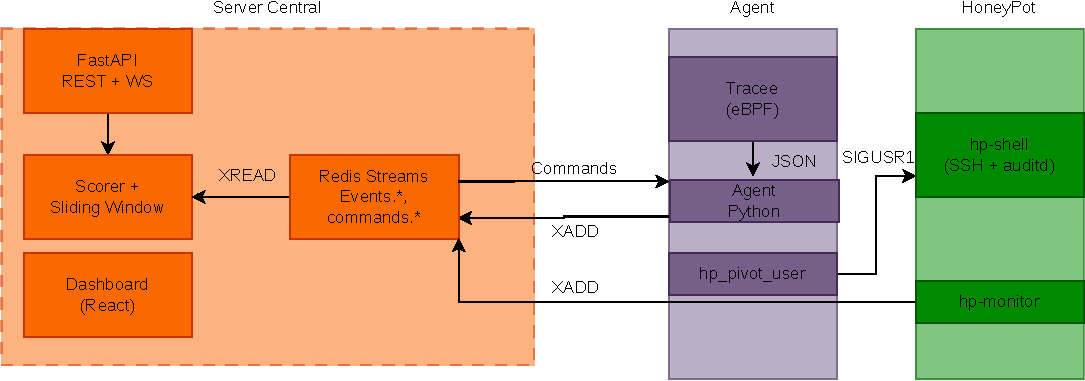
\includegraphics[width=\textwidth]{figuri/cap5-arch.pdf}
  \caption[Arhitectura de componente]{Arhitectura de componente. Cele trei zone comunică
           exclusiv prin Redis Streams; serverul central agregă fluxurile,
           atribuie scoruri și emite comenzi de pivotare.}
  \label{fig:cap5-arch}
\end{figure}

\textbf{Fluxul de pivotare.} Diagrama de secvență din figura~\ref{fig:cap5-seq-pivot}
urmărește calea completă a unui eveniment, de la momentul în care Tracee
îl captează pe gazdă, până la momentul în care shell-ul atacatorului este
înlocuit cu o sesiune SSH către container. Sunt evidențiate patru tranziții
cheie: publicarea evenimentelor în loturi pe magistrală, atribuirea scorurilor și
agregarea în fereastra glisantă, emiterea comenzii de pivotare către gazda
afectată și, în final, execuția pe gazdă a scriptului de pivotare, care
realizează în paralel trei sub-acțiuni: blocarea conexiunilor cu
\texttt{iptables}, provizionarea contului oglindit în container și trimiterea
semnalului \texttt{SIGUSR1} care comută efectiv sesiunea.

\begin{figure}[h]
  \centering
  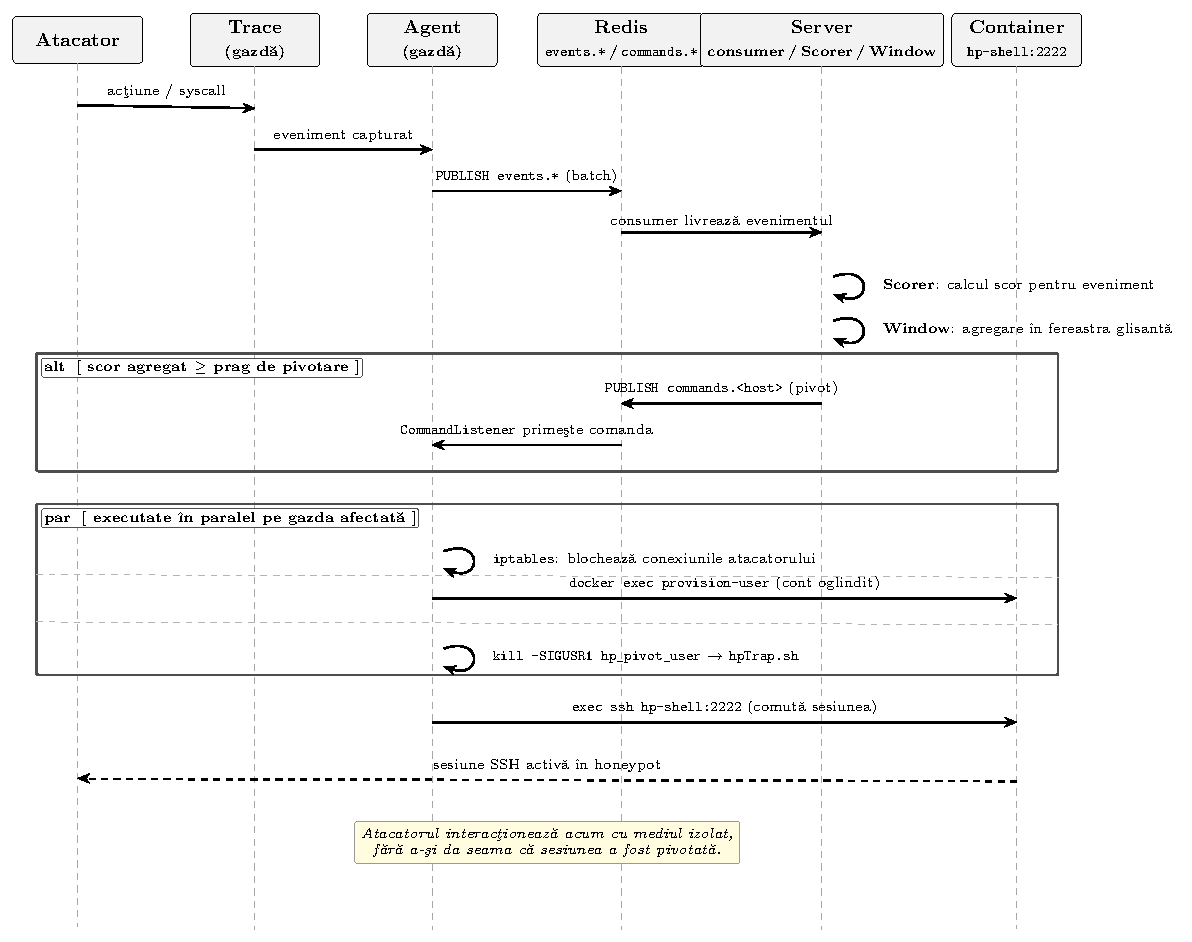
\includegraphics[width=\textwidth]{figuri/cap5-seq-pivot.pdf}
  \caption{Diagrama de secvență a procesului de detecție și pivotare}
  \label{fig:cap5-seq-pivot}
\end{figure}

\textbf{Distribuția scorurilor de normalitate.} Pentru fiecare eveniment,
modelul Isolation Forest emite un scor continuu: valorile pozitive corespund
comportamentului considerat normal, iar cele negative anomaliilor (cu cât
scorul este mai aproape de $-1$, cu atât evenimentul este mai izolat de
restul datelor benigne văzute la antrenare). Figura~\ref{fig:cap5-scores}
ilustrează distribuția acestor scoruri pe partiția de calibrare, cu cele
două praguri marcate vertical: percentila 2,0\% ($s = -0{,}022$, severitate~1)
și percentila 0,2\% ($s = -0{,}102$, severitate~2). Cele trei zone rezultate
(benign, minor și major) corespund direct nivelurilor de severitate pe baza
cărora fereastra glisantă cumulează indicii și decide când să declanșeze
pivotarea.

\begin{figure}[h]
  \centering
  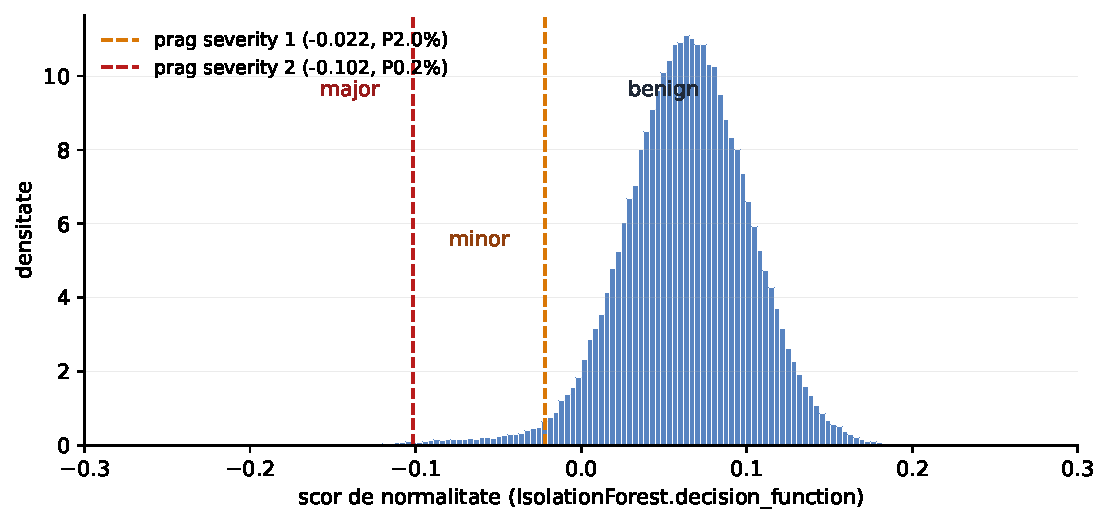
\includegraphics[width=0.85\textwidth]{figuri/cap5-scores.pdf}
  \caption[Distribuția scorurilor Isolation Forest]{Distribuția ilustrativă a scorurilor de normalitate produse de
           IsolationForest, cu pragurile de severitate 1 și 2 marcate.}
  \label{fig:cap5-scores}
\end{figure}


\section{Implementare}


\subsection{Tehnologii și organizarea proiectului}

Sistemul este împărțit în patru componente software, fiecare adaptată 
rolului pe care îl ocupă (tabelul~\ref{tab:cap5-stack}).
Alegerile principale sunt motivate de cerințele nefuncționale: framework-ul
web FastAPI împreună cu serverul \texttt{uvicorn} oferă concomitent un API
REST și un canal WebSocket asincron pe aceeași conexiune; biblioteca
scikit-learn pune la dispoziție o implementare matură și bine optimizată
a algoritmului Isolation Forest; Tracee permite instrumentarea kernelului
prin eBPF fără să fie nevoie de recompilarea pe fiecare versiune de kernel
țintă, iar Redis Streams oferă o magistrală de mesaje persistentă, suficient de
robustă pentru cazurile de utilizare ale sistemului, fără a impune
complexitatea operațională a unui sistem dedicat de mesagerie de tip Kafka
sau RabbitMQ.

\begin{table}[h]
  \centering
  \caption{Stiva tehnologică pe componente}
  \label{tab:cap5-stack}
  \renewcommand{\arraystretch}{1.08}
  \begin{tabular}{|l|l|}
    \hline
    \textbf{Componentă} & \textbf{Tehnologii} \\
    \hline\hline
    Agent de colectare        & Python 3, Tracee (\texttt{aquasec/tracee:latest}), \texttt{redis-py} \\
    \hline
    Server central            & Python 3, FastAPI, uvicorn, scikit-learn, NumPy \\
    \hline
    Container honeypot        & Docker (Ubuntu 22.04), OpenSSH, \texttt{auditd}, \texttt{util-linux} \\
    \hline
    Panou de control          & React 19, Vite 5, WebSocket \\
    \hline
    Mesagerie                 & Redis 7 (Streams) \\
    \hline
    Container runtime         & Docker (\texttt{docker.io}) \\
    \hline
  \end{tabular}
\end{table}

Repository-ul este organizat pe componente, cu două scripturi de instalare 
care ascund detaliile de inițializare:

\begin{lstlisting}[caption={Structura repository-ului (esențială)}, label={lst:cap5-tree}]
KernelTrap/
  central_server/         # Serverul central FastAPI + scorer + window
    main.py, scorer.py, window_v3.py, requirements.txt
  masina_invata/
    isolation_forest/     # Antrenare Isolation Forest pe BETH
    logger/               # Agentul (syscall_logger.py)
  Honeypot/               # Imagine Docker honeypot + script pivotare
    Dockerfile, hp_pivot_user.sh, hpTrap.sh
    provision-user.sh, record-session.sh, start-sshd.sh
    hp-monitor.py, install.sh
  dashboard/              # Aplicatie React + Vite (panoul de control)
  start_server.sh         # Bootstrap server central + Redis + dashboard
  start_agent.sh          # Bootstrap agent pe gazda monitorizata
\end{lstlisting}

\subsection{Componente}

\textbf{Agentul} este componenta care rulează pe fiecare gazdă protejată.
Primește în timp real evenimentele de syscall capturate de Tracee, le aduce
într-un format uniform (inclusiv conversia numelor de syscall în identificatori
numerici stabili, pentru a putea fi tratate consistent de modelul de
învățare automată) și le trimite serverului central în loturi, prin magistrala
Redis. Pentru a reduce zgomotul, păstrează doar evenimentele provenite de la
utilizatori conectați activ prin SSH și elimină propriile sale apeluri.
Un al doilea fir de execuție așteaptă în paralel comenzi de la server: când
primește o decizie de pivotare, lansează scriptul corespunzător pentru a
redirecționa sesiunea atacatorului în honeypot. La nivel de implementare,
toată această logică este concentrată în
\texttt{masina\_invata/logger/syscall\_logger.py}, cu clasele
\texttt{TraceeParser} (parsing) și \texttt{CommandListener} (firul de
ascultare a comenzilor), folosind biblioteca \texttt{redis-py} pentru
comunicația cu magistrala.

\textbf{Serverul central} este creierul sistemului: agregă fluxurile de la
toți agenții, atribuie un scor fiecărui eveniment și decide când o sesiune
trebuie pivotată. Activitatea este împărțită în patru sarcini care rulează
în paralel: prima consumă evenimentele primite de la agenți, a doua le atribuie un scor
și actualizează fereastra glisantă, a treia publică deciziile de pivotare înapoi
către gazde, iar ultima menține panoul de control la zi prin WebSocket.
Modulele care implementează aceste responsabilități sunt
\texttt{central\_server/main.py} (orchestrarea celor patru sarcini asincrone
peste un server FastAPI), \texttt{central\_server/scorer.py} (clasa
\texttt{Scorer}, care încapsulează modelul Isolation Forest împreună cu
pipeline-ul celor 22 de caracteristici și lexicoanele de procese
cunoscute) și \texttt{central\_server/window\_v3.py} (clasa
\texttt{SlidingWindowTracker}, care aplică pragul dublu cantitate + rată).
Modelul antrenat salvat în trei fișiere
(\texttt{iforest.joblib}, \texttt{scaler.joblib}, \texttt{meta.json}) este
încărcat în memorie o singură dată la pornire, dintr-un director versionat
împreună cu sursa.

\textbf{Mecanismul de pivotare} traduce o decizie a serverului în acțiunea
concretă de redirecționare a sesiunii atacatorului. Este realizat din două
scripturi shell complementare. Primul, \texttt{hp\_pivot\_user.sh} (instalat
în \texttt{/usr/local/sbin} cu o regulă \texttt{sudoers} care permite agentului
să-l ruleze fără parolă), execută în ordine trei acțiuni: blochează
conexiunile noi de la IP-ul atacatorului printr-o regulă \texttt{iptables},
provizionează contul corespunzător în containerul honeypot prin
\texttt{docker exec provision-user.sh}, apoi trimite semnalul
\texttt{SIGUSR1} către shell-urile active ale utilizatorului. Al doilea,
\texttt{hpTrap.sh}, este livrat ca fragment din \texttt{/etc/profile.d/}
și se încarcă automat în fiecare shell interactiv la login; instalează un
\textit{trap} care, la primirea semnalului \texttt{SIGUSR1}, înlocuiește
procesul curent al shell-ului cu o sesiune SSH către container, fără ca
utilizatorul să observe tranziția:

\begin{lstlisting}[caption={Trap-ul instalat în fiecare shell interactiv (\texttt{hpTrap.sh})}, label={lst:cap5-trap}]
hptrap_pivot() {
  logger -t hptrap "Pivoting user $USER from host to honeypot"
  exec ssh -i /etc/hptrap/hp_key -o StrictHostKeyChecking=no \
    "${USER}@127.0.0.1" -p 2222
}
trap hptrap_pivot USR1
\end{lstlisting}

\textbf{Containerul honeypot} oferă un mediu Linux aparent obișnuit, în
care atacatorul ajunge după pivotare. Imaginea de bază este \texttt{ubuntu:22.04}
cu server SSH, auditare la nivel de kernel (\texttt{auditd}) și utilitarele
uzuale de linie de comandă. La momentul pivotării, un script de
provizionare creează automat în container un cont oglindit (cu același nume
ca pe gazda reală) și populează directorul home al acestuia cu fișiere-momeală
plauzibile: chei AWS, o cheie SSH privată, un fișier de mediu cu credențiale
fictive de bază de date, note interne și un token CI/CD. Toate aceste fișiere
sunt urmărite de \texttt{auditd}: orice citire sau scriere asupra lor generează
imediat un eveniment. Pe lângă canary-uri, sesiunea integrală a atacatorului
este înregistrată ca tranzit TTY, iar un script de monitorizare
(\texttt{hp-monitor.py}) citește continuu log-ul \texttt{auditd} și publică
evenimentele înapoi pe magistrala Redis, în același format folosit de agenții
de pe gazdele reale, astfel încât panoul de control le poate afișa unitar,
indiferent de sursă.

\textbf{Panoul de control} este o aplicație web scrisă în React, păstrată
deliberat minimală (singurele dependențe runtime sunt \texttt{react} și
\texttt{react-dom}). Comunică cu serverul central pe două căi: un API REST
pentru date relativ statice (lista agenților, istoric pivotări) și o conexiune
WebSocket pentru fluxul live de evenimente. Reconectarea automată cu
\textit{backoff} exponențial (creșterea progresivă a intervalului dintre
încercări) este gestionată centralizat printr-un singur \textit{hook}
custom, astfel încât celelalte componente pot presupune că au date la zi.
Vizual, panoul este împărțit în patru zone: lista agenților conectați
(\texttt{AgentsPanel}), fluxul de log-uri în timp real (\texttt{LiveLogs}),
tabelul utilizatorilor monitorizați cu progresul în fereastra glisantă
(\texttt{UsersTable}) și istoricul pivotărilor (\texttt{PivotHistory}).
Aplicația este compilată ca site static și servită direct de serverul
FastAPI, eliminând nevoia unui server web separat.

\textbf{Antrenarea modelului} se realizează offline, înainte de punerea
în funcțiune a sistemului, pe partiția benignă a setului de date BETH.
Pentru a putea folosi întregul volum de date disponibil (zeci de gigabytes),
fără a-l încărca complet în memorie, se folosește o tehnică de eșantionare
numită \textit{reservoir sampling}: pe măsură ce datele sunt citite în
\textit{streaming}, un eșantion uniform de dimensiune fixă este menținut și
actualizat probabilistic. Concret, modelul folosit în producție este antrenat
pe 10 milioane de instanțe astfel eșantionate, cu o pădure de 2000 de arbori
de izolare. Pragurile de severitate 1 și 2 nu sunt fixate arbitrar, ci sunt
calibrate ulterior pe o partiție de validare, alegând percentilele 2,0\% și
0,2\% ale scorurilor de normalitate, astfel încât proporția de evenimente
marcate ca anomalii pe date benigne să fie controlată explicit. Aceste praguri,
împreună cu tabelele de codificare prin frecvență ale câmpurilor categoriale,
sunt salvate în \texttt{meta.json} și citite la pornirea serverului central.
Scriptul de antrenare se află în
\texttt{masina\_invata/isolation\_forest/beth\_iforest.py}.


\section{Testare}


Sistemul a fost validat prin cinci tipuri complementare de testare,
descrise pe scurt mai jos. Rezultatele cantitative în special cele
referitoare la detecția scenariilor reale de atac sunt prezentate detaliat
în capitolul~\ref{tab:cap6-perf}.

\textbf{Testarea modelului de învățare automată.} Scriptul de antrenare
expune o subcomandă dedicată de evaluare care încarcă modelul deja antrenat
împreună cu partiția de test a setului BETH, calculează scorurile, aplică
pragurile de severitate calibrate și raportează două metrici de referință
asupra atacurilor etichetate: aria de sub curba ROC (\texttt{roc\_auc\_evil})
și precizia medie (\texttt{avg\_precision\_evil}). Acest test este reluat
la fiecare reantrenare, ca o regresie de calitate care semnalează imediat
dacă o nouă versiune a modelului pierde din capacitatea de detecție.

\textbf{Teste unitare pe componentele critice ale serverului.} Cele două
clase cu logică algoritmică sensibilă \texttt{Scorer} și
\texttt{SlidingWindowTracker} sunt acoperite de teste unitare \texttt{pytest}
(\texttt{tests/test\_scorer.py} și \texttt{tests/test\_window.py}). Pentru
\texttt{Scorer} sunt verificate încărcarea corectă a modelului,
schema evenimentelor procesate și comportamentul pe input
degenerat (lot gol). Pentru \texttt{SlidingWindowTracker} sunt verificate
condițiile fundamentale ale pragului dublu: nici un pivot sub prag, pivotare
exact când cantitatea și rata sunt simultan satisfăcute, blocarea pivotării
când rata este sub limită (chiar dacă numărul de evenimente severe e mare),
ignorarea UID-urilor omise și suprimarea pivotărilor repetate imediat
după un pivot deja declanșat.

\textbf{Testare de integrare end-to-end.} Cea mai relevantă verificare
practică se face prin rulări controlate ale întregului sistem: pornirea
simultană a serverului central (\texttt{start\_server.sh}) și a agentului
pe o gazdă de test (\texttt{start\_agent.sh}), generarea manuală de
activitate (autentificare SSH, comenzi controlate de recon) și observarea
în panoul de control că evenimentele apar, primesc scor, fereastra glisantă
cumulează severitățile și, la pragul atins, pivotarea este efectiv
declanșată. O singură astfel de rulare exersează magistrala Redis Streams
în ambele direcții, scoring-ul, fereastra glisantă și mecanismul de pivotare.

\textbf{Testarea mecanismului de pivotare și a honeypot-ului.} Pivotarea
este verificată suplimentar prin invocare directă din linia de comandă:
\texttt{sudo hp\_pivot\_user <username>} într-o sesiune SSH activă.
Se confirmă apariția regulii \texttt{iptables} (vizibilă cu
\texttt{iptables -L INPUT -n}), tranziția shell-ului către container
(PID-ul shell-ului inițial este înlocuit) și prezența fișierelor-momeală
în directorul home oglindit. Înregistrarea integrală a sesiunii este
verificată prin inspecția fișierelor din \texttt{/var/log/sessions/} ale
containerului, iar regulile de auditare sunt validate prin acces deliberat
la fișierele-capcană și observarea evenimentelor corespunzătoare în panou.

\textbf{Testarea panoului de control.} Interfața web este verificată
manual în browser: indicatorul de status al serverului (verde/roșu),
fluxul de evenimente prin WebSocket, tabelul utilizatorilor cu progresul
ferestrei glisante și declanșarea unui pivot prin butonul dedicat.
Reconectarea automată cu \textit{backoff} exponențial este verificată prin
oprirea voluntară a serverului în timpul rulării panoului clientul se
reconectează la repornirea serverului, fără intervenție manuală.

Această combinație a fost preferată unei suite extinse de teste unitare pe
toate componentele: întrucât sistemul este distribuit și comunică exclusiv
prin Redis Streams, comportamentul realist apare doar la integrare. Testele
unitare au fost menținute strict acolo unde logica este suficient de izolată
și de critică pentru a justifica izolarea în Scorer și în fereastra glisantă 
iar restul componentelor sunt acoperite de testele de integrare end-to-end.


% ================================================================
% Capitolul 6 – Evaluare
% Lucrare de licență: Kernel Trap – Sistem Inteligent de Prevenire
% a Intruziunilor cu Componente de Honeypot și Învățare Automată
% Autor: Banciu George-Horațiu
% Coordonator: Conf. Univ. Dr. Bufnea Darius Vasile
% ================================================================

\chapter{Evaluare}

Capitolul de față prezintă evaluarea experimentală a sistemului KernelTrap.
Sunt enunțate, mai întâi, asumările de securitate pe care se sprijină
funcționarea corectă a sistemului; sunt apoi raportate metricile de
performanță măsurate pe mediul de testare, urmate de trei scenarii concrete
de atac executate cu unelte folosite curent în comunitatea de securitate
ofensivă; secțiunea finală tratează limitările sistemului și clasele de
atacatori pe care îi acoperă cu eficacitate maximă.

% ----------------------------------------------------------------
\section{Asumări de securitate}
% ----------------------------------------------------------------

KernelTrap este un sistem de prevenire a intruziunilor proiectat pentru un
scenariu specific: un cont SSH neprivilegiat compromis pe o gazdă altfel
necompromisă. Validitatea protecției oferite depinde de două asumări fundamentale
asupra mediului de rulare, sintetizate în tabelul \ref{tab:cap6-trust}.

\begin{table}[h]
  \centering
  \caption{Asumările de securitate ale sistemului}
  \label{tab:cap6-trust}
  \renewcommand{\arraystretch}{1.08}
  \begin{tabular}{|p{0.32\textwidth}|p{0.58\textwidth}|}
    \hline
    \textbf{Asumare} & \textbf{Consecință} \\
    \hline\hline
    Contul \texttt{root} nu este compromis.
      & Agentul, scriptul de pivotare, regulile \texttt{iptables} și controlul containerului honeypot rulează cu privilegii ridicate. Un atacator care a obținut deja drepturi \texttt{root} poate dezactiva agentul, șterge regulile de firewall, opri procesul de scoring sau modifica însăși logica de pivotare. \\
    \hline
    Atacatorul nu are acces fizic la mașină.
      & Atacuri prin consola fizică (\texttt{tty*}), dispozitive USB ostile, modificare hardware, reset GRUB sau extragere de disc cad în afara domeniului de aplicabilitate. Filtrarea agentului pe sesiuni SSH \texttt{pts/*} reflectă explicit această alegere. \\
    \hline
  \end{tabular}
\end{table}

Din aceste asumări derivă două consecințe operaționale: telemetria colectată
prin eBPF/Tracee este considerată de încredere atâta timp cât kernelul
însuși nu este compromis; iar scriptul de pivotare, deși expus pentru a
putea fi rulat fără parolă de către agent (printr-o regulă \texttt{sudoers}
de tip \texttt{NOPASSWD} aplicată strict pe comanda \texttt{hp\_pivot\_user}),
nu este proiectat să reziste unui atacator care a obținut deja drepturi
de modificare a fișierelor de sistem.

% ----------------------------------------------------------------
\section{Mediul de testare și metodologie}
% ----------------------------------------------------------------

Configurația folosită pentru evaluare este descrisă în tabelul
\ref{tab:cap6-env}. Topologia a constat dintr-o gazdă monitorizată, serverul
central de analiză și containerul honeypot, rulate pe aceeași subrețea
locală pentru a izola măsurătorile de variabilitatea WAN.

\begin{table}[h]
  \centering
  \caption{Configurația mediului de testare}
  \label{tab:cap6-env}
  \renewcommand{\arraystretch}{1.08}
  \begin{tabular}{|l|p{0.55\textwidth}|}
    \hline
    \textbf{Componentă} & \textbf{Configurație} \\
    \hline\hline
    Gazda monitorizată       & TODO: <distribuție Linux, kernel, CPU, RAM>  \\
    \hline
    Serverul central         & TODO: <distribuție, RAM, CPU>                \\
    \hline
    Container honeypot       & Docker (Ubuntu 22.04), capabilități \texttt{AUDIT\_WRITE}, \texttt{AUDIT\_CONTROL} \\
    \hline
    Versiune Tracee          & \texttt{aquasec/tracee:latest} (TODO: <commit/tag>) \\
    \hline
    Versiune Python          & TODO: <3.x>                                   \\
    \hline
    Versiune Redis           & 7 (imagine oficială Docker)                   \\
    \hline
  \end{tabular}
\end{table}

Evaluarea a vizat două categorii de proprietăți: (1) overhead-ul de
performanță introdus pe gazda monitorizată, în repaus și în regim de lucru;
(2) capacitatea de detecție pe trei scenarii cu unelte publice de atac.

% ----------------------------------------------------------------
\section{Performanță}
% ----------------------------------------------------------------

Tabelul \ref{tab:cap6-perf} sintetizează metricile măsurate pe mediul descris
mai sus, raportate la țintele nefuncționale enunțate în capitolul 5
(tabelul \ref{tab:cap5-nfr}).

\begin{table}[h]
  \centering
  \caption{Metrici de performanță}
  \label{tab:cap6-perf}
  \renewcommand{\arraystretch}{1.08}
  \begin{tabular}{|l|l|l|l|}
    \hline
    \textbf{Metrică} & \textbf{Valoare} & \textbf{Țintă} & \textbf{Verdict} \\
    \hline\hline
    CPU agent (idle)                          & TODO: \texttt{<X\%>}  & < 2,5\% (NF1) & TODO \\
    \hline
    CPU agent                                 & TODO: \texttt{<X\%>}  & < 2,5\% (NF1) & TODO \\
    \hline
    RAM agent                                 & TODO: \texttt{<X> MB} & ---           & ---  \\
    \hline
    RAM server central                        & TODO: \texttt{<X> MB} & ---           & ---  \\
    \hline
    Throughput susținut server                & TODO: \texttt{<X> ev/s} & ---         & ---  \\
    \hline
  \end{tabular}
\end{table}

% ----------------------------------------------------------------
\section{Scenarii de atac și răspunsul sistemului}
% ----------------------------------------------------------------

Pentru a verifica capacitatea de detecție pe acțiuni cu profil realist, au
fost executate trei scenarii pe gazda monitorizată, după autentificarea unui
cont SSH neprivilegiat. Fiecare scenariu este descris prin succesiunea de
acțiuni ale atacatorului, indicatorii observați de KernelTrap și verdictul
sistemului.

\subsection{Scenariul 1: recon automat cu LinPEAS}

LinPEAS este un script Bash open-source folosit pe scară largă pentru
enumerarea automată a căilor de privilege escalation pe sisteme Linux. La
execuție lansează în cascadă zeci de procese pentru colectarea de informații
despre sistem, conturi, configurări de servicii și permisiuni.

\begin{table}[h]
  \centering
  \caption{Scenariul 1: indicatori observați la rularea LinPEAS}
  \label{tab:cap6-scen1}
  \renewcommand{\arraystretch}{1.08}
  \begin{tabular}{|p{0.42\textwidth}|p{0.48\textwidth}|}
    \hline
    \textbf{Acțiunea atacatorului} & \textbf{Indicator KernelTrap} \\
    \hline\hline
    \texttt{wget}/\texttt{curl} script de pe host extern   & \texttt{is\_network\_tool=1}, \texttt{has\_url\_or\_ip=1} \\
    \hline
    \texttt{id}, \texttt{whoami}, \texttt{uname}, \texttt{hostname}, \texttt{ss}, \texttt{ps} în cascadă & \texttt{is\_basic\_recon=1} repetat \\
    \hline
    Citire \texttt{/etc/passwd}, \texttt{/etc/shadow}, \texttt{.ssh/}      & \texttt{has\_sensitive\_path=1} \\
    \hline
    Rafale dense de syscall-uri          & \texttt{syscall\_rate\_5s} și \texttt{unique\_syscalls\_5s} ridicate \\
    \hline
  \end{tabular}
\end{table}

Rezultat: severitatea 2 apare pe majoritatea evenimentelor în primele
secunde de execuție; fereastra glisantă atinge pragul dublu
(cantitate $\geq$ 5 și rată $\geq$ 30\%) și emite comanda de pivotare.

\subsection{Scenariul 2: stabilirea unui canal C2 cu Sliver}

Sliver este un framework C2 open-source modern, similar conceptual cu
Cobalt Strike, folosit în testele de penetrare și în campanii reale de
post-exploatare. Scenariul a constat din descărcarea implantului Sliver
pe gazda compromisă, marcarea executabilă și pornirea acestuia; implantul
a deschis o conexiune outbound persistentă către serverul C2, iar
operatorul a emis remote comenzi standard de recon.

\begin{table}[h]
  \centering
  \caption{Scenariul 2: indicatori observați la setup Sliver}
  \label{tab:cap6-scen2}
  \renewcommand{\arraystretch}{1.08}
  \begin{tabular}{|p{0.42\textwidth}|p{0.48\textwidth}|}
    \hline
    \textbf{Acțiunea atacatorului} & \textbf{Indicator KernelTrap} \\
    \hline\hline
    Fetch implant (\texttt{curl}/\texttt{wget})              & \texttt{is\_network\_tool=1}, \texttt{has\_url\_or\_ip=1} \\
    \hline
    Pornire implant cu nume custom                          & \texttt{processName\_freq=0} (necunoscut datelor BETH) \\
    \hline
    Conexiune persistentă către C2 (\texttt{connect}, \texttt{sendto}, \texttt{recvfrom})  & \texttt{syscall\_rate\_5s} susținut pe socket non-standard \\
    \hline
    Comenzi remote: \texttt{id}, \texttt{sudo -l}, \texttt{whoami}  & \texttt{is\_basic\_recon=1}, \texttt{is\_privileged\_helper=1} \\
    \hline
  \end{tabular}
\end{table}

Rezultat: combinația dintre processName cu frecvență zero, indicatorii de
rețea și comenzile remote scor-uite ca recon împinge fereastra peste
ambele praguri. Pivotarea automată redirecționează sesiunea SSH activă
către containerul honeypot, iar regula \texttt{iptables} adăugată pe IP-ul
C2 blochează stabilirea oricăror conexiuni noi de la același atacator.

\subsection{Scenariul 3: acces la fișiere canary post-pivotare}

După redirecționarea în honeypot, atacatorul (sau implantul automat al
acestuia) explorează directorul home al utilizatorului oglindit și
încearcă să citească fișiere ce par să conțină credențiale: chei AWS
(\texttt{.aws/credentials}), cheie privată SSH (\texttt{.ssh/id\_rsa}),
fișier de mediu cu credențiale de bază de date (\texttt{.env}), note interne
(\texttt{notes.txt}) și un token de CI/CD (\texttt{.jenkins\_token}).
Pentru fiecare astfel de acces, regulile \texttt{auditd} instalate de
\texttt{provision-user.sh} emit câte un eveniment, captat de
\texttt{hp-monitor.py} și publicat pe stream-ul Redis al containerului.

\begin{table}[h]
  \centering
  \caption{Scenariul 3: indicatori observați la accesul canary}
  \label{tab:cap6-scen3}
  \renewcommand{\arraystretch}{1.08}
  \begin{tabular}{|l|l|}
    \hline
    \textbf{Fișier canary accesat}     & \textbf{Indicator KernelTrap} \\
    \hline\hline
    \texttt{\textasciitilde/.aws/credentials} & \texttt{has\_canary\_path=1}, regulă \texttt{audit\_001} \\
    \hline
    \texttt{\textasciitilde/.ssh/id\_rsa}     & \texttt{has\_canary\_path=1}, regulă \texttt{audit\_002} \\
    \hline
    \texttt{\textasciitilde/.env}              & \texttt{has\_canary\_path=1}, regulă \texttt{audit\_003} \\
    \hline
    \texttt{\textasciitilde/notes.txt}         & regulă \texttt{audit\_004}  \\
    \hline
  \end{tabular}
\end{table}

Rezultat: spre deosebire de detecția probabilistică din scenariile
precedente, accesul la fișiere canary constituie un indicator binar de
compromitere, niciun utilizator legitim nu are motiv să deschidă aceste
fișiere, întrucât conțin credențiale fictive plasate intenționat ca
momeală. Indicatorii apar imediat în panoul de control și confirmă
post-factum că pivotarea a fost justificată, oferind în plus telemetrie
asupra credențialelor pe care atacatorul le urmărește.

% ----------------------------------------------------------------
\section{Limitări}
% ----------------------------------------------------------------

Această secțiune enunță explicit clasele de atac pe care sistemul nu le
acoperă eficient. Scopul este de a delimita responsabilitatea KernelTrap și
de a evita așteptări nerealiste asupra protecției oferite.

\textbf{Atacatori avansați cu unelte proprii.} Un actor de tip APT
(\textit{Advanced Persistent Threat}, atacator cu resurse și obiective de
nivel statal sau corporativ) care folosește binare scrise sau modificate
de el însuși poate ocoli o parte din indicatorii sistemului. Două categorii
de tehnici sunt în mod special problematice. Prima: nume de proces alese
deliberat pentru a semăna cu daemoni legitimi de sistem (de exemplu, un
implant numit \texttt{kworker/0:1} sau \texttt{systemd-resolved-helper})
păcălește codificarea prin frecvență a câmpului \texttt{processName} și
lexicoanele de procese cunoscute. A doua: tehnici care nu lasă deloc urma
caracteristică a unei comenzi noi, adică cod executat direct din memorie, fără
ca un proces nou să fie creat prin syscall-ul \texttt{execve} (\textit{fileless});
injectarea unei biblioteci dinamice ostile într-un proces deja existent și
benign (\textit{DLL/SO injection} în \texttt{sshd} sau \texttt{bash});
sau interpunerea pe syscall-urile unui proces de încredere prin
\texttt{ptrace} (un mecanism de depanare folosit pentru a controla execuția
altui proces). Aceste tehnici sunt caracteristice operatorilor cu resurse
considerabile și nu constituie profilul de atacator țintă al sistemului.

\textbf{Atacuri pre-autentificare.} Agentul monitorizează exclusiv UID-urile
cu sesiuni SSH interactive active (terminalele virtuale \texttt{pts/*}).
În consecință, ies complet din raza sa de acoperire: brute-force-ul SSH
(încercări automate de parole care nu produc o sesiune validă), exploit-urile
care vizează direct procesul \texttt{sshd} înainte de stabilirea sesiunii,
precum și atacurile asupra altor servicii expuse public (servere web,
baze de date).

\textbf{Exploit de kernel sau orbire a Tracee.} Un atac care reușește să
dezactiveze sau să modifice programele eBPF deja încărcate în kernel orbește
complet agentul. Aceasta poate veni dintr-o vulnerabilitate
\textit{zero-day} în verificatorul eBPF (componenta de kernel care validează
programele eBPF înainte de încărcare), din exploatarea capabilităților
privilegiate \texttt{CAP\_BPF} sau \texttt{CAP\_SYS\_ADMIN}, sau din
înlocuirea pur și simplu a binarului Tracee. Toate aceste tehnici necesită
oricum drepturi apropiate de \texttt{root}, situație în care protecția
oferită se reduce la asumarea explicită din secțiunea~\ref{tab:cap6-trust}
(contul \texttt{root} este considerat necompromis).

\textbf{Vectori de atac în afara SSH.} Execuția de cod la distanță printr-o
aplicație web compromisă (\textit{Remote Code Execution} pe Apache, Tomcat,
servere de aplicații), sarcini malițioase rulate prin \texttt{cron}, sau
exploit-uri ale unor servicii care rulează sub conturi de sistem alb-listate
(\texttt{www-data} pentru servere web, \texttt{mysql}, \texttt{postgres}
pentru baze de date) sunt invizibile filtrelor agentului, întrucât nu trec
prin nicio sesiune SSH. KernelTrap este construit pentru scenariul „cont
SSH neprivilegiat compromis", nu pentru compromiterea generală a tuturor
serviciilor expuse.

\subsection{Domeniul de aplicabilitate optim}

Pentru a clarifica unde KernelTrap oferă valoare maximă, tabelul
\ref{tab:cap6-fit} cartografiază principalele profile de atacator
împotriva nivelului de acoperire al sistemului.

\begin{table}[h]
  \centering
  \caption{Profile de atacator și acoperirea KernelTrap}
  \label{tab:cap6-fit}
  \renewcommand{\arraystretch}{1.08}
  \begin{tabular}{|p{0.34\textwidth}|c|p{0.42\textwidth}|}
    \hline
    \textbf{Profil atacator} & \textbf{Acoperire} & \textbf{Motiv} \\
    \hline\hline
    Script kiddies / atacatori oportuniști                 & Optimă   & Folosesc kit-uri publice (LinPEAS, LinEnum, pspy, module recon Metasploit) ușor recunoscute prin lexicoane. \\
    \hline
    Botneturi care compromit SSH prin credential stuffing  & Optimă   & După obținerea foothold-ului, execută în lanț scripturi automate de post-exploatare (recon, descărcare payload, persistență, lateral movement); generează rafale dense de syscall-uri și procese cu profil zgomotos, ușor de prins de fereastra glisantă. \\
    \hline
    Mișcare laterală prin cont SSH compromis              & Optimă   & Scenariul de proiectare; întreaga arhitectură este construită pentru acest caz. \\
    \hline
    APT cu tooling custom / fileless / 0-day kernel        & Limitată & Indicatorii bazați pe nume de proces și syscall-uri standard nu rețin profilul. \\
    \hline
    Brute-force / exploit pre-autentificare                & Niciuna  & Filtrele pe UID SSH activ exclud această fază. \\
    \hline
    RCE prin aplicații web sau servicii expuse             & Niciuna  & UID-urile sistemice sunt alb-listate; vectorul nu trece prin SSH. \\
    \hline
  \end{tabular}
\end{table}

KernelTrap își propune să ridice semnificativ costul atacatorilor de nivel
mediu segmentul în care se încadrează majoritatea atacurilor observate în
trafic real, conform sondajelor de threat intelligence fără a pretinde
acoperirea spectrului complet pe care un EDR enterprise îl tratează.

% ----------------------------------------------------------------
\section{Sinteză evaluare}
% ----------------------------------------------------------------

Evaluarea experimentală a confirmat că sistemul atinge ținta de
overhead stabilită în capitolul 5 (sub 2,5\% pe CPU pe gazda monitorizată)
și detectează cu succes atât tooling-ul de recon automat (LinPEAS), cât și
stabilirea unui canal C2 modern (Sliver), declanșând în fiecare caz
pivotarea automată a sesiunii SSH compromise.
Indicatorii binari de tip canary, observați după redirecționarea în
honeypot, oferă confirmarea independentă a faptului că pivotarea a fost
justificată și telemetrie suplimentară asupra obiectivelor atacatorului.
Limitările identificate actori avansați cu tooling custom, atacuri
pre-autentificare, vectori în afara SSH sunt asumate explicit și
poziționează KernelTrap ca un sistem de detecție și răspuns activ
specializat pe atacatori autentificați de nivel mediu, complementar
soluțiilor de protecție perimetrale și EDR-urilor generale, nu un
înlocuitor pentru acestea.


\chapter{Concluzii și direcții viitoare}

Lucrarea de față a tratat problema integrării a două abordări complementare de
apărare cibernetică (detecția intruziunilor pe gazdă și honeypot-urile) într-un
singur sistem care detectează automat un atacator autentificat prin SSH și îl
redirecționează transparent într-un mediu izolat. Capitolul 2 a introdus
fundamentele teoretice necesare: apelurile de sistem ca sursă de telemetrie,
tehnologia eBPF cu instrumentul Tracee, algoritmul Isolation Forest, magistrala
Redis Streams și containerele Docker. Capitolul 3 a analizat stadiul actual,
acoperind sistemele HIDS bazate pe eBPF, metodele de învățare automată
nesupervizată aplicate la detecția intruziunilor, honeypot-urile SSH cu
interacțiune ridicată și mecanismele de apărare activă. Pe baza analizei,
capitolul 4 a propus arhitectura sistemului KernelTrap și a justificat fiecare
decizie de proiectare în raport cu literatura citată. Capitolul 5 a prezentat
implementarea celor patru componente decuplate (agent, server central, container
honeypot, panou de control) și modul lor de comunicare prin Redis Streams.
În fine, capitolul 6 a raportat evaluarea experimentală pe trei scenarii reale
de atac, metricile de performanță măsurate și limitările asumate explicit.

Revenind la promisiunile enunțate în introducere, lucrarea confirmă livrarea
celor trei niveluri funcționale anunțate. Colectarea evenimentelor de syscall
prin eBPF cu Tracee a fost concretizată în agentul descris în subsecțiunea
\textit{Componente} a capitolului 5. Analiza centralizată cu un model Isolation
Forest antrenat pe setul de date BETH a fost concretizată în clasa
\texttt{Scorer} a serverului central, calibrată prin praguri obținute pe partiția
de validare. Mecanismul de răspuns activ, adică combinația de semnal POSIX, regulă
\texttt{iptables} și provizionare în container Docker, a fost concretizat în
scripturile \texttt{hp\_pivot\_user.sh} și \texttt{hpTrap.sh}. Pivotarea
transparentă, fără alertarea atacatorului, a fost demonstrată în cele trei
scenarii reale din capitolul 6 (recon automat cu LinPEAS, stabilirea unui
canal C2 cu Sliver, accesul la fișiere canary post-pivotare), iar ținta de
overhead stabilită ca cerință nefuncțională (sub 2,5\% pe CPU) a fost atinsă.

Limitările sistemului (atacatori APT cu unelte proprii, atacuri
pre-autentificare, exploit-uri de kernel și vectori în afara SSH) au fost
asumate explicit în secțiunea omonimă a capitolului 6 și nu reprezintă o
omisiune, ci o decizie deliberată privind domeniul de aplicabilitate. KernelTrap
nu pretinde acoperirea spectrului complet de atacuri, ci abordarea eficientă
a unei clase bine definite: atacatorul autentificat de nivel mediu pe o gazdă
altfel sănătoasă.

Pe partea de direcții viitoare, sistemul construit reprezintă o bază solidă
pe care se pot construi mai multe extinderi naturale, dintre care cele mai
promițătoare sunt următoarele:

\begin{enumerate}
  \item \textbf{Detecție hibridă: semnături combinate cu comportament.}
    Combinarea modelului Isolation Forest cu un strat de reguli declarative
    (Sigma, YARA) ar permite acoperirea simultană a două categorii de atac:
    cele cunoscute, capturate cu precizie ridicată de semnături, și cele
    necunoscute sau anomale, capturate de model. Stratul de semnături poate
    funcționa ca o cale rapidă care scurtcircuitează scoringul ML atunci când
    un tipar cunoscut este recunoscut, reducând atât latența cât și rata de
    fals pozitive.

  \item \textbf{Honeypot configurabil per scenariu.}
    Containerul honeypot este în prezent o imagine Ubuntu generică, cu un
    set fix de fișiere-momeală. O extindere naturală constă în introducerea
    de profile selectabile (server web cu fișiere de configurare Nginx
    fictive, server de baze de date cu dumpuri SQL momeală, workstation de
    dezvoltare cu repository-uri Git ce conțin credențiale inserate
    intenționat), alese automat în funcție de profilul gazdei monitorizate
    sau de comportamentul observat al atacatorului.

  \item \textbf{Extindere către o suită HIPS / NIPS / EDR.}
    KernelTrap acoperă în prezent doar stratul HIPS, axat pe gazdă. O
    direcție de dezvoltare semnificativă ar fi adăugarea unui modul NIPS
    (\textit{Network Intrusion Prevention System}) care să analizeze fluxul
    de pachete dintre agenți, respectiv a unor capabilități tipice EDR
    (\textit{Endpoint Detection and Response}) precum monitorizarea
    integrității fișierelor critice de sistem și jurnalizarea per-proces
    a accesului la fișiere sensibile.

  \item \textbf{Corelare cross-host pentru detecția mișcării laterale.}
    Arhitectura curentă tratează fiecare gazdă independent; un atacator
    care pivotează succesiv prin mai multe servere generează semnale
    separate, fără o vedere unificată. Adăugarea unui modul de corelare pe
    serverul central, care să grupeze evenimente după identitate (cheie
    SSH reutilizată, IP sursă, proximitate temporală), ar permite detecția
    pattern-urilor de tip multi-step intrusion și emiterea unei comenzi de
    pivotare simultan pe toate gazdele afectate.

  \item \textbf{Integrare cu surse externe de threat intelligence.}
    Conectarea sistemului la feed-uri publice de tip MISP sau AlienVault OTX
    ar permite popularea automată a blocklist-urilor \texttt{iptables} cu
    IP-uri ostile cunoscute și îmbogățirea panoului de control cu context
    suplimentar (categoria atacatorului, campanie atribuită, indicatori
    asociați). În plus, datele colectate în propriul honeypot ar putea fi
    publicate înapoi în feed-uri, contribuind la ecosistemul de partajare.

  \item \textbf{Honeypot augmentat cu modele lingvistice (arie de cercetare).}
    O direcție exploratorie este utilizarea modelelor lingvistice mari (LLM)
    pentru generarea dinamică a răspunsurilor în honeypot (ieșiri credibile
    la \texttt{cat}, \texttt{ls} sau \texttt{ps}), făcând mediul-momeală
    mai convingător pentru atacatorii umani. Lucrări recente, precum cea
    a lui Sladić et al.~\cite{sladic2024llm}, explorează această direcție și
    pot oferi un punct de plecare pentru o eventuală integrare.
\end{enumerate}

În sinteză, lucrarea de față a contribuit cu un sistem distribuit funcțional
care demonstrează fezabilitatea integrării detecției comportamentale cu un
răspuns activ izolant, oferind atât o platformă utilizabilă în practică pe
gazde Linux protejate, cât și un punct de plecare concret pentru extinderile
enumerate mai sus. KernelTrap se poziționează astfel ca o componentă
complementară soluțiilor perimetrale și EDR-urilor enterprise, nu ca un
înlocuitor pentru acestea.

\bibliographystyle{plain}
\bibliography{references}

\end{document}